%%%% Version 6. Condensed, publication-ready revision of main_v5.tex (v5 was 27 pp).
%%%%
%%%% Page budget, measured rather than estimated (sn-jnl, iicol):
%%%%   body 21 pp + references 6 pp = 27 pp. Text and tables alone occupy 17 pp and the
%%%%   eleven figure floats add 4 pp, so an 18-pp body would have had room for roughly
%%%%   three of the thirteen figures. Kye's call (2026-08-17) was to keep every figure
%%%%   and accept ~21 pp of body; references are excluded from the target.
%%%%
%%%% What changed relative to v5:
%%%%   * Every fact of v5 is retained; what is removed is repetition. v5 stated most of
%%%%     its headline numbers four times (abstract, results, discussion, conclusion).
%%%%     Numbers now live in the Results and the tables, the Discussion interprets them
%%%%     without restating them, and the Conclusion carries only what a reader must leave
%%%%     with. Mechanical parameters moved from prose into Tables 1 and 2.
%%%%   * All 13 figures are retained. Four are paired into two-panel floats (setup +
%%%%     sample flow; confusion + per-participant) and the t-SNE moves to a single column.
%%%%     Float-packing parameters are tuned below: default LaTeX fractions stranded about
%%%%     a page in placement dead space with this many full-width floats.
%%%%   * Tables 4 and 5 of v5 (aggregate and per-class five-class performance) are merged.
%%%%   * The bibliography moves to BibTeX (refs.bib) and grows from 21 to 89 entries.
%%%%     NOTE: sn-jnl already issues \bibstyle{sn-nature}; do NOT add \bibliographystyle.
%%%%     sn-nature.bst mishandles @inproceedings, so conference papers are entered as
%%%%     @article with the proceedings name in `journal`.
%%%%   * RQ3 gains the deep-baseline arm (Table 7). Run baselines_emg_only_20260816
%%%%     completed 2026-08-17 05:50, 60/60 folds. THE PROPOSED MODEL DOES NOT WIN IT:
%%%%     dual_branch_temporal_cnn reaches 75.0 % macro-F1 against the wavelet CNN's
%%%%     72.2 %, consistently across seeds but on three of five participants and at
%%%%     3x the parameters. Reported as measured; see sec:deep_baselines and the
%%%%     Discussion paragraph in "The classification finding". Whether to promote the
%%%%     temporal CNN to the headline model is Kye's open decision -- it would mean
%%%%     regenerating Figs 6-8, 10 and 12 from its checkpoints.
%%%%   * Section "Training behaviour and computational cost": the latency figures were
%%%%     UNSOURCED before this revision (0.95/0.97 ms appeared in no artifact) and the
%%%%     cited parameter counts belonged to the fusion variants of a pre-correction
%%%%     benchmark. Both now come from outputs/benchmarks/benchmark_emg_only.json,
%%%%     measured emg_only through the corrected chain on an idle machine.
%%%%
%%%% Every reported number comes from one of these artifacts:
%%%%   outputs/runs/modality_and_no_chewing_20260810T020642_cead62e4  (emg_only conditions)
%%%%   outputs/runs/baselines_emg_only_20260816                      (RQ3 architectures)
%%%%   outputs/screening/emg_only_filter_contrast.json                (RQ1 filter contrast)
%%%%   outputs/screening/emg_only_design.json                         (design constraints)
%%%%   outputs/screening/emg_only_contrast.json                       (RQ3 feature baselines)
%%%%   outputs/data_audit/7ebbcc8d74c0bbe0/                           (guards, sweeps, mains)
%%%%   outputs/benchmarks/benchmark.json                              (reference latencies)
%%%% Run-dependent figures live in Figures/v5/ so that main_4.tex still compiles.
\documentclass[pdflatex,sn-nature,iicol]{sn-jnl}

\usepackage{graphicx}
\usepackage{multirow}
\usepackage{amsmath,amssymb}
\usepackage{booktabs}
\usepackage{mathrsfs}
\usepackage[title]{appendix}
\usepackage{xcolor}
\usepackage{textcomp}
\usepackage{manyfoot}
\usepackage{indentfirst}

\graphicspath{{./}{figures/}{Figures/}}

%%%% Float packing. These change typesetting only -- no content is added or removed.
%%%% The default LaTeX fractions reserve so much of each page for text that a document
%%%% with 11 full-width floats strands roughly two pages in placement dead space.
\renewcommand{\topfraction}{0.92}
\renewcommand{\bottomfraction}{0.70}
\renewcommand{\textfraction}{0.06}
\renewcommand{\floatpagefraction}{0.80}
\renewcommand{\dbltopfraction}{0.92}
\renewcommand{\dblfloatpagefraction}{0.80}
\setcounter{topnumber}{3}
\setcounter{bottomnumber}{2}
\setcounter{totalnumber}{4}
\setcounter{dbltopnumber}{3}
\setlength{\floatsep}{6pt plus 2pt minus 2pt}
\setlength{\textfloatsep}{8pt plus 2pt minus 2pt}
\setlength{\dblfloatsep}{6pt plus 2pt minus 2pt}
\setlength{\dbltextfloatsep}{8pt plus 2pt minus 2pt}
\setlength{\intextsep}{6pt plus 2pt minus 2pt}

\begin{document}

\title[Audited Surface-EMG Classification of Instructed Jaw Activities]{The Measurement Chain Outweighs the Model: Audited Surface-EMG Classification of Instructed Jaw Activities Relevant to Tooth-Contact Bruxism}

\author[1]{\fnm{Mohammad Hassan} \sur{Farhadi}}
\author[1]{\fnm{Ali} \sur{Rabiee}}
\author[1]{\fnm{Rahul} \sur{Singh}}
\author[2,3]{\fnm{Mariusz P.} \sur{Furmanek}}
\author*[1]{\fnm{Reza} \sur{Abiri}}\email{reza\_abiri@uri.edu}
\author*[4]{\fnm{Theodore A.} \sur{Walls}}\email{walls@uri.edu}

\affil[1]{\orgdiv{Department of Electrical, Computer, and Biomedical Engineering}, \orgname{University of Rhode Island}, \orgaddress{\city{Kingston}, \state{RI}, \country{United States}}}
\affil[2]{\orgdiv{Department of Physical Therapy}, \orgname{University of Rhode Island}, \orgaddress{\city{Kingston}, \state{RI}, \country{United States}}}
\affil[3]{\orgdiv{Institute of Sport Sciences, Academy of Physical Education in Katowice}, \orgaddress{\city{Katowice}, \country{Poland}}}
\affil[4]{\orgdiv{Department of Psychology}, \orgname{University of Rhode Island}, \orgaddress{\city{Kingston}, \state{RI}, \country{United States}}}

\abstract{Instrumental studies of masticatory-muscle activity are reported almost entirely through summary accuracies, and the measurement chain that produced them is rarely auditable. On 100 awake laboratory recordings from five adults with a prior clinical diagnosis of bruxism, we show that this chain can outweigh every modelling choice made on top of it. A spectral audit found that the acquisition hardware had already suppressed the 60-Hz mains fundamental and that the surviving interference was harmonic: 62 recordings carried more than 30\% of their raw in-band electromyographic power within $\pm3$~Hz of a mains multiple, rising to 91.3--99.8\% in the five dedicated quiet-rest recordings. The conventional recipe---notch the fundamental, then band-pass---removed the one frequency that was absent and passed everything that was present. Replacing it with a constant-width harmonic notch bank moved a matched nested leave-one-subject-out (LOSO) network from 43.5\% to 72.8\% participant-level macro-F1 on byte-identical windows, folds and labels, and two far simpler classifiers by 22 to 27 points; quiet-rest false alarms fell fivefold, the between-participant amplitude spread nearly halved, and two participants who had been unclassifiable moved into the normal range. What had looked like severe between-participant heterogeneity was largely interference. On the corrected signal, a compact wavelet convolutional network with 5,901 parameters (23.1~KiB) separated quiet rest, jaw movement, clenching, instructed grinding and chewing at 81.7\% accuracy, 72.0\% macro-F1 and a macro one-vs-rest ROC--AUC of 0.958 under leakage-free nested LOSO, with quiet rest the best-recalled class and 7.7\% of quiet-rest windows falling on the tooth-contact side of a collapsed clenching/grinding split. The learned representation beat hand-engineered band energies on identical windows---an advantage that did not exist before the correction---and beat two larger learned baselines, although a variant able to represent burst--relaxation rhythm beat it in turn; normalisation scope and temporal context each proved worth more than the architecture. A microphone was also recorded, as an annotation aid; a channel-integrity audit found it unusable and it is not analysed. These results establish technical feasibility for this five-participant dataset and, more durably, a reporting practice: publish a measured interference statistic beside every accuracy, and draw filter responses over the measured spectrum of the recordings rather than alone.}

\keywords{Jaw-activity classification, Surface electromyography, Convolutional neural networks, Wavelet decomposition, Powerline interference, Signal-quality audit, Measurement validity, Leave-one-subject-out validation}

\maketitle

\section{Introduction}

Instrumental assessment of masticatory-muscle activity outside the clinic is a sensing and classification problem before it is anything else. Surface electromyography (EMG) measures masticatory activation directly and is the standard modality for ambulatory recording~\cite{raez2006techniques,colonna2023electromyographic,thymi2021signal}, but it responds similarly to functional and non-functional activity: clenching, grinding and chewing all produce sustained or bursting masseter and temporalis activation, and a one-second window of one can resemble a window of another. Whether a compact learned model can separate those conditions from each other and from quiet rest, on participants it has never seen, is one of the questions this paper measures.

It is not the first one. Studies in this area are reported almost exclusively through summary accuracies, and the measurement chain that produced them is rarely auditable~\cite{thymi2021signal,cidverdejo2024instrumental}. A spectral audit of our own recordings, run during the preparation of this analysis, showed that the conventional preprocessing recipe applied to them---notch the mains fundamental, then band-pass---removed the one frequency the acquisition hardware had already suppressed and left the mains \emph{harmonics}, which carried the overwhelming majority of the in-band power, entirely intact. A filter-response plot of that chain looks textbook-correct. Nothing in the pipeline was untested, unversioned or irreproducible; the defect was invisible because no figure had ever placed the filter response over the measured spectrum of the data.

Correcting it changed the results by more than every other intervention we evaluated combined. That is the organising claim of this paper, and it is stated first because it reorders what is worth reporting: a classifier trained through a defective channel can appear to work while separating interference rather than physiology, and leave-one-subject-out (LOSO) evaluation is precisely the protocol that then reports the consequence as poor generalisation across people. We therefore report the audit, the correction, its measured effect on classification, and only then the classifier that runs on the corrected signal.

\paragraph{Scope.} Two statements follow from current terminology and are made here once. International consensus defines bruxism as masticatory-muscle activity that may involve clenching or grinding with tooth contact, or bracing and thrusting without it, and distinguishes sleep from awake manifestations~\cite{lobbezoo2013bruxism,lobbezoo2018international,verhoeff2025definitions,manfredini2022bruxism}. Tooth contact is therefore neither necessary for all bruxism activities nor sufficient to establish that an observed activity is bruxism. Second, every activity analysed here was performed on instruction in a laboratory: the class names used below---rest, movement, clenching, grinding and chewing---denote experimental conditions, and a classifier that separates them is not a diagnostic device~\cite{manfredini2024standardised}. The study does not evaluate spontaneous awake bruxism, sleep bruxism, severity or treatment response, and neither point is revisited later.

\paragraph{Research questions.} \textbf{RQ1:} how much does the mains-interference correction change what a classifier can learn from these recordings, measured on identical windows and folds? \textbf{RQ2:} on the corrected signal, can four channels of surface EMG and a compact wavelet convolutional network distinguish quiet rest from four instructed jaw activities, under a protocol in which no held-out participant's data touch any fitted quantity? \textbf{RQ3:} does the learned wavelet representation classify better than hand-engineered band-energy features, and better than alternative learned architectures, under that same protocol? Results obtained before the filter correction are superseded and are not restated for comparison: the two sets of numbers were measured through different measurement chains on the same recordings.

\section{Prior technical advances}

\subsection{EMG-based assessment of masticatory activity}

Surface EMG is widely used for ambulatory assessment because it measures masticatory activation directly~\cite{raez2006techniques,farella2008masticatory}. Bruxism itself is common, heterogeneous and difficult to observe directly~\cite{lavigne2008bruxism,manfredini2013epidemiology,melo2019bruxism,wetselaar2019prevalence}, and its reference standards are demanding: polysomnography with audio--video recording remains the standard for sleep bruxism~\cite{lavigne1996sleep,stuginski2016detection}, while portable instruments show variable agreement with it~\cite{casett2017validity,cidverdejo2024instrumental}. Awake bruxism is assessed mainly by ecological momentary assessment rather than by any instrument~\cite{bracci2018frequency,zani2019ecological}, which is part of why an instrumental awake measure is worth developing. Early portable EMG systems established the feasibility of home recording but had limited specificity for distinguishing target activity from other orofacial activity~\cite{stuginski2016detection}. Castroflorio et al.~\cite{castroflorio2013use,castroflorio2014detection} combined EMG and electrocardiographic information to identify sleep-bruxism episodes in a natural environment; multi-day home recording has since been shown to be feasible~\cite{colonna2023electromyographic}, and consensus guidance now exists for ambulatory EMG in this setting~\cite{lobbezoo2020consensus}.

Machine-learning studies report high performance on controlled tasks, although direct comparison is difficult when labels, participants and validation protocols differ. Sonmezocak and Kurt~\cite{sonmezocak2021detection} reported greater than 90\% accuracy from EMG features across jaw opening, clenching, rhythmic grinding and fatigue/pain classes; Gul et al.~\cite{gul2024advanced} evaluated sleep-related recordings across postures; Heyat et al.~\cite{heyat2020computational} combined several physiological modalities; and Lan et al.~\cite{lan2022comparative} described different surface-EMG patterns during centric and eccentric instructed activities. Alternative sensing routes include mandibular-movement analysis for phasic sleep bruxism~\cite{martinot2021artificial}, chin-mounted accelerometry~\cite{patwa2017bruxism}, contingent-stimulation devices~\cite{haugland2020automatic} and head-mounted acoustic transducers, whose output depends strongly on placement~\cite{romano2024wearable}. These studies support technical feasibility but do not make their accuracies interchangeable: some classify pre-segmented tasks whereas others identify events within continuous recordings, and portable devices intended for sleep require comparison with an appropriate reference method~\cite{cidverdejo2024instrumental}.

\subsection{Signal processing and learned representations}

Wavelet decomposition suits non-stationary EMG because it preserves joint time--frequency information~\cite{mallat1989theory,daubechies1992ten,englehart2003robust}, and wavelet features perform well in EMG classification~\cite{phinyomark2012feature,bharathi2025unveiling}. Filter design remains important for preserving physiological content while suppressing noise~\cite{chowdhury2013surface,deluca2010filtering,clancy2002sampling,merletti2020tutorial,boyer2023reducing}, and the useful band for facial, jaw and neck muscles has been measured directly~\cite{vanboxtel2001optimal}. Recording standards and consensus matrices exist for electrode selection and amplitude normalisation~\cite{isek1999standards,hermens2000development,besomi2019consensus,besomi2020consensus,merletti2019tutorial,deluca1997use}. Convolutional networks learn local patterns in physiological signals~\cite{faust2018deep,craik2019deep,tsinganos2019improved,rim2020deep,kiranyaz20211d,ismailfawaz2019deep}, an approach mature enough in myoelectric control to have public benchmarks~\cite{atzori2014electromyography,atzori2016deep,coteallard2019deep,jiang2012myoelectric,phinyomark2018emg,wei2019multistream}, and focal loss and class weighting reduce the influence of class imbalance~\cite{lin2017focal,johnson2019survey}.

\subsection{The gap this paper addresses}

Surface-EMG reviews consistently identify powerline interference as the dominant environmental artifact and recommend notch filtering combined with a band-pass stage~\cite{chowdhury2013surface,raez2006techniques}. That recommendation is usually implemented as a single notch at the supply frequency, which is valid only when the supply fundamental is in fact the dominant interference; harmonic-aware and subtraction-based alternatives exist but are rarely used in this literature~\cite{mewett2004reducing,levkov2005removal,keshtkaran2014fast,sornmo2005bioelectrical}. Head-mounted electrodes with long leads, in a laboratory containing displays, lighting and switched-mode supplies, can instead pick up a harmonic-rich waveform, and some acquisition systems apply their own fixed notch before the data reach the analysis software. In that combination the textbook chain removes nothing and still looks correct on a filter-response plot.

The gap is therefore not a missing architecture. It is that published accuracies in this literature are almost never accompanied by a measured statement about the signal they were computed from---a scoping review of ambulatory EMG for bruxism found acquisition and analysis parameters reported inconsistently or not at all~\cite{thymi2021signal}---so a reader cannot tell whether a reported number describes physiology or interference. The same concern drives reporting standards and leakage audits elsewhere in clinical machine learning~\cite{collins2024tripod,kapoor2023leakage,varoquaux2022machine,pineau2021improving}. Verifying the filter against the measured spectrum of the actual recordings, rather than against its own design, is cheap, and it is the step this paper adds and then prices.

\section{Methods}

This proof-of-concept study was approved by the Institutional Review Board of the University of Rhode Island (Protocol \#IRB22275690-2) and performed in accordance with relevant institutional guidelines and regulations. Written informed consent was obtained from every participant, including consent to publish the identifying image in Fig.~\ref{fig:setup}a.

\subsection{Participants, procedure and sensors}

Five adults (2 women and 3 men; age $38.0 \pm 10.4$ years) were recruited through flyers, messages to local oral-care and physical-therapy providers, and word of mouth; eligibility required a prior clinical diagnosis of bruxism. The study did not independently re-diagnose or phenotype that history, and the available records did not stratify participants by sleep bruxism, awake bruxism, grinding, bracing or thrusting predominance. The prior diagnosis therefore describes the sample and is not a reference standard for the activity labels used here. All analysed tasks were performed intentionally while participants were awake in the laboratory; no spontaneous episodes and no sleep were recorded.

Each session began with written consent and a pre-screening survey, after which surface-EMG electrodes, an omnidirectional microphone and a camera were positioned and secured. Participants completed 1 minute of quiet rest, then five repetitions each of jaw opening/closing, left/right deviation, protrusion/retrusion and left/right biting, then 1-minute trials of isometric molar and incisor clenching alternating 3 seconds of activity with 3 seconds of relaxation. After a break they completed 3-minute trials of instructed grinding, chewing cheese, chewing baby carrots or popcorn, and chewing gum. Each task was repeated three times with a 1-minute rest between repetitions. A handheld button transmitted event markers synchronised with the physiological recordings: participants pressed it at task initiation and the experimenter visually confirmed onset.

Four differential surface-EMG channels were recorded from two bilateral bipolar electrode pairs, one per side of the head (Fig.~\ref{fig:setup}a); the tentative electrode map records them as left masseter, left temporalis, right masseter and right temporalis, the sites for which bilateral surface recording and its reproducibility are best characterised~\cite{ferrario2000electromyographic,castroflorio2005reproducibility}. All signals were sampled at 1200~Hz. The acquisition chain documented no physical calibration, so all amplitudes are reported in arbitrary analog-to-digital converter units and are deliberately not labeled \textmu V, and electrode type, amplifier, preamplifier gain and converter resolution are not documented. This falls short of current reporting recommendations~\cite{isek1999standards,besomi2019consensus} and is stated so that the omission is visible rather than inferred.

\begin{figure*}[t]
  \centering
  \raisebox{0.03\height}{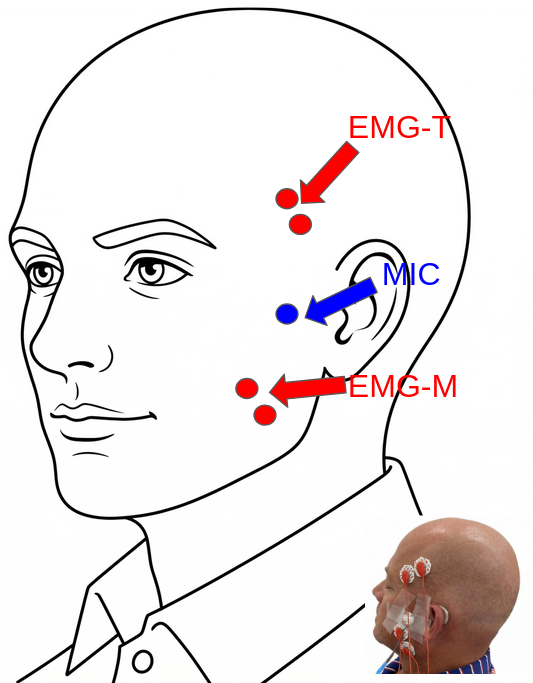
\includegraphics[width=0.195\linewidth]{Figures/patient_new.png}}\hfill
  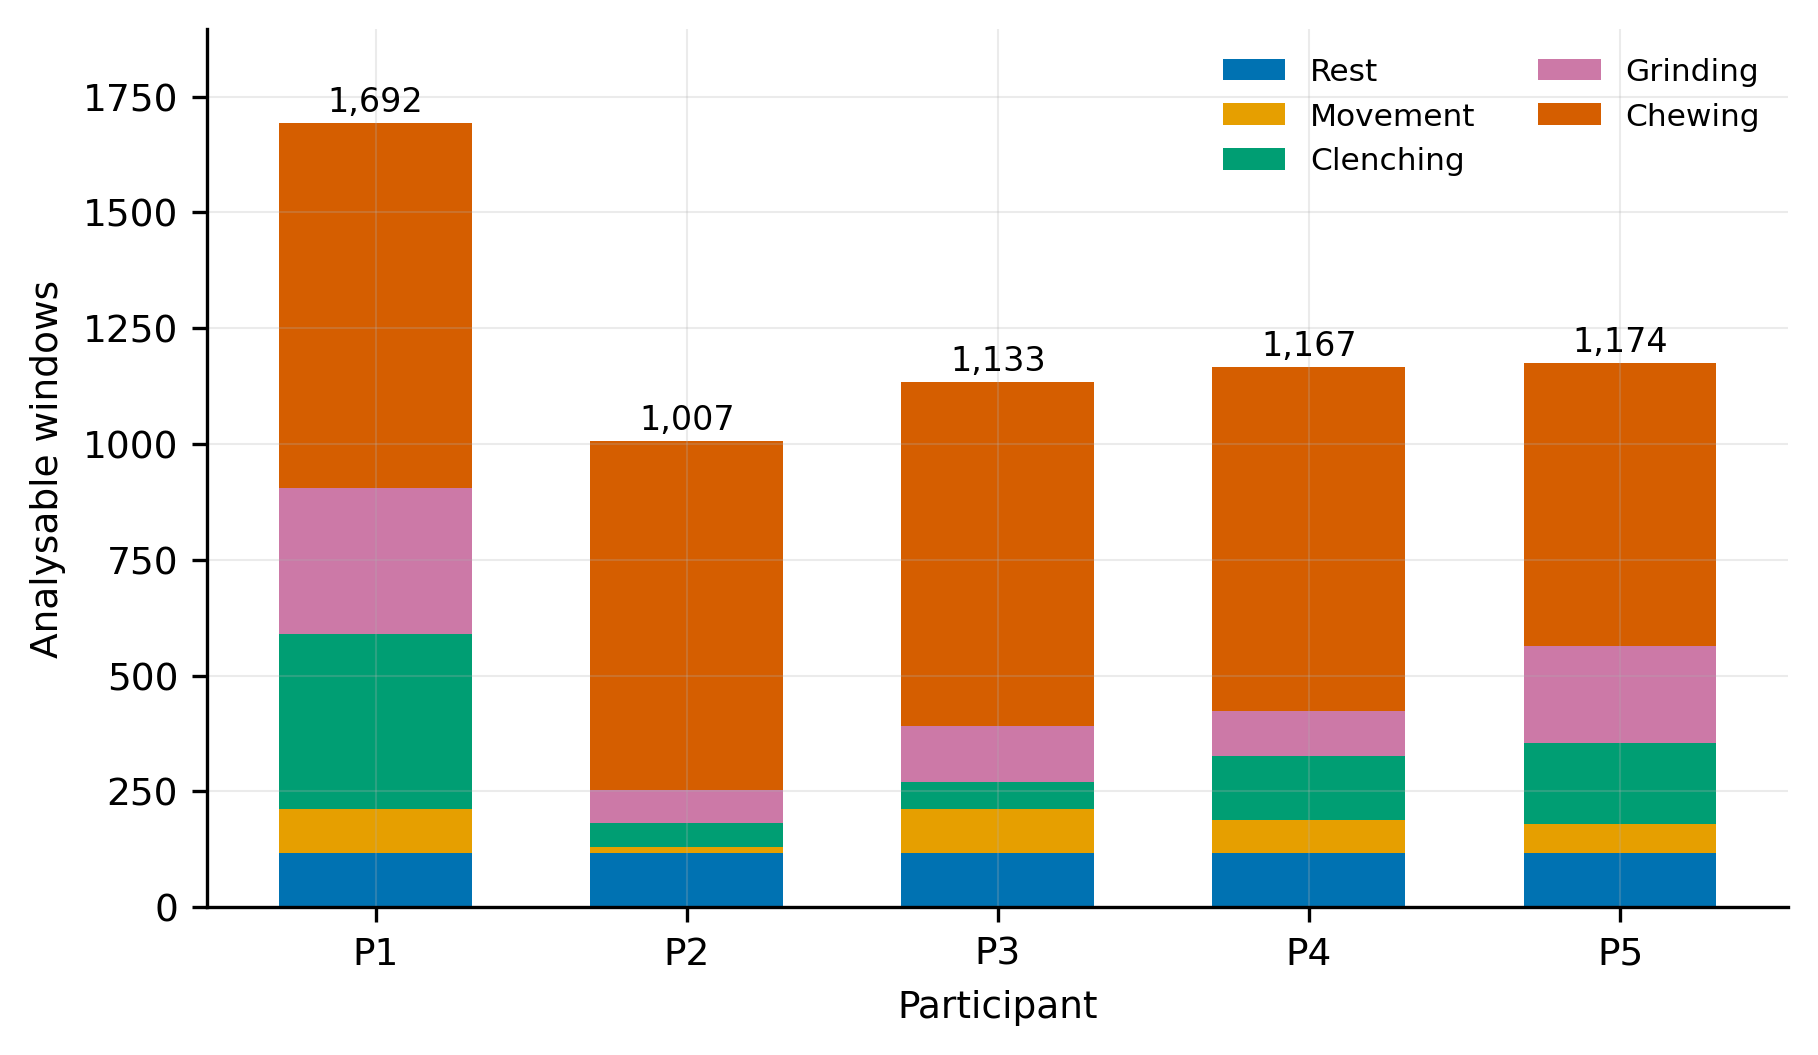
\includegraphics[width=0.600\linewidth]{Figures/v5/sample_flow.png}
  \caption{The study. (a) Sensor placement: bipolar surface-EMG pairs over the temporalis (EMG-T) and masseter (EMG-M), with a microphone (MIC) near the temporomandibular joint as an annotation aid; it is not analysed, for the measured reasons in Section~\ref{sec:mic}. (b) Analysable windows per participant and class after the containment, transition-guard and startup-guard exclusions; participants are labelled P1--P5 here and throughout. Class sizes are strongly unequal both between classes---chewing supplies 58.9\%---and between participants within a class, which is why class weighting, minority-only augmentation and participant-level aggregation are all used; Section~\ref{sec:constraints} traces the between-participant inequality to how differently participants marked the trigger.}
  \label{fig:setup}
\end{figure*}

\subsection{Window labelling and the analysable sample}
\label{sec:windows}

Every analysed window lies \emph{wholly inside} one interval during which the trigger marks the participant as actively performing the named task, so no window can span two conditions or a trigger transition. Windows are cut from the continuously filtered recording and never filtered individually, because filtering each window separately injects an edge transient exceeding one signal standard deviation into its first 50 samples.

Three exclusions are applied before windowing, and each guard was measured rather than assumed (Table~\ref{tab:dataset}). A \textbf{transition guard} of 0.25~s is removed on each side of every trigger edge: over 432 task onsets, 358 of them with a detectable envelope transition, the median lag between button press and electromyographic onset was $-0.075$~s and muscle activity preceded the marker at 79.9\% of onsets, while among the 20\% of onsets in the harmful direction the median lag was 0.054~s and the largest measured was 0.352~s. A \textbf{startup guard} of 0.5~s is removed at the beginning of every recording, replacing an earlier unexplained 3-s skip; amplifier settling transients appeared in 66 of 100 recordings, all settled within 0.40~s, with peak excursions up to $12{,}580\times$ the recording's robust scale. Finally, quiet-rest windows are drawn only from the five dedicated rest recordings, because trigger-off intervals inside active recordings are unlabelled rather than verified as quiet. The rest class therefore represents quiet laboratory rest, not the full range of everyday non-event behaviour.

The recordings were consolidated into five experimental classes. \textbf{Rest} comprised windows from the five dedicated quiet-baseline recordings only; \textbf{movement} included opening/closing, lateral deviation and protrusion/retrusion; \textbf{clenching} included molar clench, incisor clench and unilateral left/right bite; \textbf{grinding} included the instructed grinding trials; and \textbf{chewing} included cheese, carrots or popcorn, and gum. These categories contrast quiet non-event periods, non-chewing jaw movement, static loading, lateral tooth-contact activity and functional mastication; bracing and thrusting without tooth contact were not elicited and are not represented. Chewing was included because it is a common functional activity and a plausible confound for an ambulatory jaw-activity classifier, and because it may also be comparatively easy to recognise, the primary five-class results are accompanied by a sensitivity analysis that excludes it and by a second that collapses the five labels into instructed clenching/grinding versus rest/movement/chewing.

Under these rules, 100 recordings yielded 6,173 analysable 1.0-second windows from 99 recordings (Table~\ref{tab:dataset}, Fig.~\ref{fig:setup}b). These counts supersede the 11,845 windows reported previously, which a legacy policy produced by labelling whole recordings rather than trigger-verified intervals and which therefore included inter-trial and transition material inside activity classes; the two sets are not comparable. The windows are not independent observations---adjacent windows overlap by 50\%, many come from the same recording, and all come from five people---so the participant, not the window, is the effective unit for generalisation, and all primary metrics are computed within a participant before being summarised~\cite{saeb2017need,little2017using,roberts2017cross}.

\begin{table}[t]
  \caption{Dataset, guards and preprocessing under the trigger-constrained labelling policy.}
  \label{tab:dataset}
  \centering
  \footnotesize
  \begin{tabular*}{\columnwidth}{@{\extracolsep{\fill}}ll@{}}
    \toprule
    Property & Value \\
    \midrule
    Participants / recordings & 5 / 100 (99) \\
    EMG channels analysed & 4 (2 bilateral pairs) \\
    Microphone channels analysed & 0 (rec., excluded) \\
    Sampling rate / units & 1200 Hz / arbitrary ADC \\
    Window / stride & 1200 (1.0 s) / 600 (0.5 s) \\
    Transition guard, per edge & 0.25 s \\
    Startup guard, per recording & 0.5 s \\
    \midrule
    Rest windows (5 dedicated recs.) & 590 \\
    Movement windows & 333 \\
    Clenching windows & 799 \\
    Grinding windows & 816 \\
    Chewing windows & 3,635 \\
    \textbf{Total analysed windows} & \textbf{6{,}173} \\
    \midrule
    Mains notches (8 Hz wide) & 60--420 Hz, 7 harm. \\
    Band-pass (Butterworth, order 4) & 20--450 Hz \\
    Filtering mode & Zero-phase, whole rec. \\
    Wavelet / bands & db4, 4 lev.\ / $A_4$, $D_3$, $D_1$ \\
    \bottomrule
  \end{tabular*}
\end{table}

\subsection{Mains interference and the corrected filter chain}
\label{sec:filter}

Every result in this paper was regenerated after a spectral audit of the raw recordings. Because that audit is the subject of RQ1, its measurements are given here and its effect on classification in Section~\ref{sec:rq1}.

The acquisition software applied its own fixed notch, recorded in every metadata sidecar, and that notch removed the 60-Hz fundamental before the data reached disk. Interference survived at the harmonics instead. Measured against the local noise floor of the raw signals, the peaks at 180, 300 and 420~Hz ranged from tens of times that floor in the least affected participant to more than a million times it in the most affected. Across all 100 recordings, 62 had more than 30\% of their raw in-band EMG power within $\pm 3$~Hz of a mains multiple, and in the five dedicated quiet-rest recordings that share was 91.3--99.8\%.

The chain used in earlier analyses of this dataset was a single 60-Hz notch ($Q=30$) followed by a 20--450-Hz band-pass. On these recordings it removed the only mains frequency that was already absent and passed every frequency that was present: the mains share of in-band power after filtering was 91.4--99.8\%, essentially unchanged from the raw signal (Fig.~\ref{fig:filter_fix}a, c). A filter-response plot of that chain looks entirely conventional, which is why the problem stayed invisible until the response was drawn over the measured spectrum of the data.

The corrected chain notches every mains multiple inside the pass band---60, 120, 180, 240, 300, 360 and 420~Hz---before the same fourth-order Butterworth band-pass from 20 to 450~Hz, a band consistent with direct measurements of the useful bandwidth of jaw and facial EMG~\cite{vanboxtel2001optimal,deluca2010filtering}. Each notch is \emph{constant-width} (8~Hz at $-3$~dB, so $Q = f_0/8$) rather than constant-$Q$, which would give a 2-Hz notch at 60~Hz and a 14-Hz notch at 420~Hz: the narrowest response exactly where the hardware notch left a residue, the widest where nothing survives. Both variants remove 56~Hz of the 430-Hz pass band, an identical 13\% cost, but at that cost the constant-width bank left the worst-contaminated cell at $3.2\times$ its local noise floor against $25.6\times$ for constant $Q$, an eight-fold reduction in residual interference; after correction the mains share in the quiet-rest recordings fell to 0.46--0.66\% (Fig.~\ref{fig:filter_fix}b, c). A comb filter and spectrum interpolation~\cite{mewett2004reducing} were also implemented and measured on the same windows; both left more residual interference, and spectrum interpolation is additionally acausal by construction.

The chain was selected on this interference criterion, which can be specified in advance, and not on held-out classification score. The distinction is not decorative: the constant-$Q$ bank scored marginally \emph{higher} in screening classification (0.689 versus 0.679 macro-F1 on the same windows) while leaving eight times the residual interference, so a score criterion would have selected it.

All filtering is zero-phase (forward--backward second-order sections) and applied to the whole continuous recording before any window is cut. Zero-phase filtering reads samples from the future of each output sample; it is appropriate for the offline analysis reported here and cannot support a streaming, wearable or real-time claim. A causal mode exists in the implementation, and the mode used is recorded in every run bundle.

\begin{figure*}[t]
  \centering
  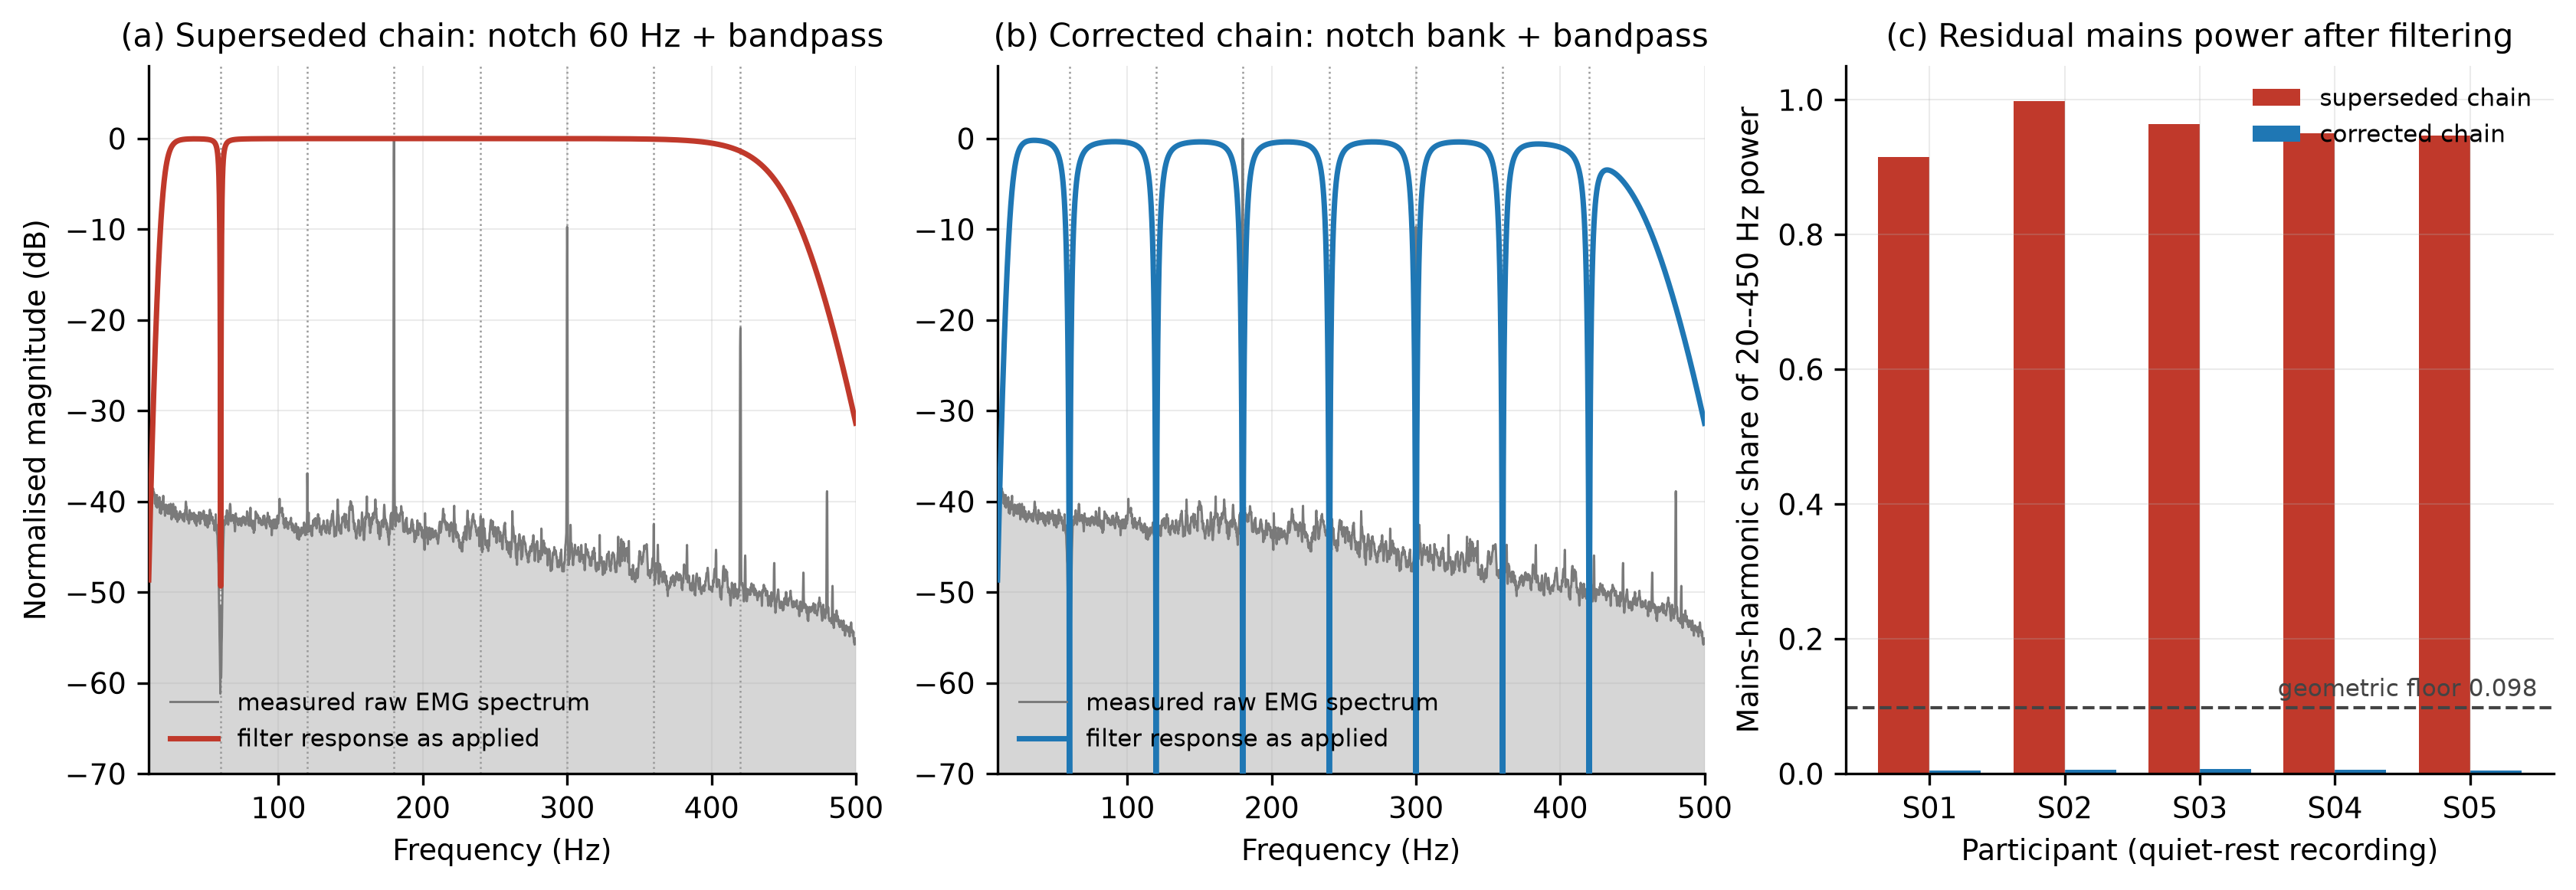
\includegraphics[width=0.86\linewidth]{Figures/filter_defect_and_correction.png}
  \caption{The mains-harmonic defect and its correction. (a) The superseded chain: the 60-Hz notch lands where the hardware had already removed the fundamental, while the tall harmonic peaks at 180, 300 and 420~Hz pass the band-pass untouched. (b) The corrected chain: seven constant-width notches land on the peaks. Gray traces are the mean raw EMG spectrum of the five quiet-rest recordings, colored traces the zero-phase response as applied, dotted lines 60~Hz and its harmonics. (c) Share of 20--450-Hz power within $\pm3$~Hz of a mains multiple, per participant, after each chain; the dashed line marks the 0.098 a white signal would score, since seven $\pm3$-Hz bands occupy 42~Hz of a 430-Hz pass band, and a notch bank scores below it by deleting those bins.}
  \label{fig:filter_fix}
\end{figure*}

\subsection{Normalisation, wavelet decomposition and model}

EMG signals were z-scored per channel using means and standard deviations computed \emph{only} from the training participants of the fold in question. The list of participants that produced each fold's statistics is stored with the fold and asserted not to contain the held-out participant before that participant is evaluated. A per-participant (transductive) scope is implemented and prespecified as a separate configuration, and Section~\ref{sec:constraints} prices it, but no confirmatory number here uses it: the strict scope is the one that would support a deployment claim without a fitting session~\cite{besomi2020consensus}.

Figure~\ref{fig:preprocessing} shows the chain on a real excerpt. Signals were then decomposed with the Daubechies-4 wavelet at four levels, and the sub-branches used $A_4$ ($<38$~Hz), $D_3$ (75--150~Hz) and $D_1$ (300--600~Hz, of which only the 300--450-Hz portion survives the band-pass). Daubechies wavelets were selected for their compact support and prior use in transient EMG analysis~\cite{daubechies1992ten,englehart2003robust}. The pipeline now rejects any band its own filter chain has removed, unless the configuration declares the exception explicitly.

The model is a single-branch wavelet convolutional network (Fig.~\ref{fig:architecture}) with three CNN sub-branches, one per retained band. Each applies a 3-tap convolution to 8 channels, batch normalisation, a rectified linear unit, max pooling by 2, a second 3-tap convolution to 16 channels, batch normalisation, a rectified linear unit and adaptive average pooling to one value per channel, contributing 16 features per band and 48 in total. Those 48 features pass to a multilayer perceptron (MLP) of dimensions $48\rightarrow48\rightarrow32$, with batch normalisation, a rectified linear unit and dropout at probability 0.5 in each hidden layer, and a final linear layer produces logits for the five classes. The complete model has 5,901 trainable parameters---1,656 in the wavelet branch, 4,080 in the MLP, 165 in the classification head---or 23.1~KiB at 32-bit precision.

\begin{figure*}[t]
  \centering
  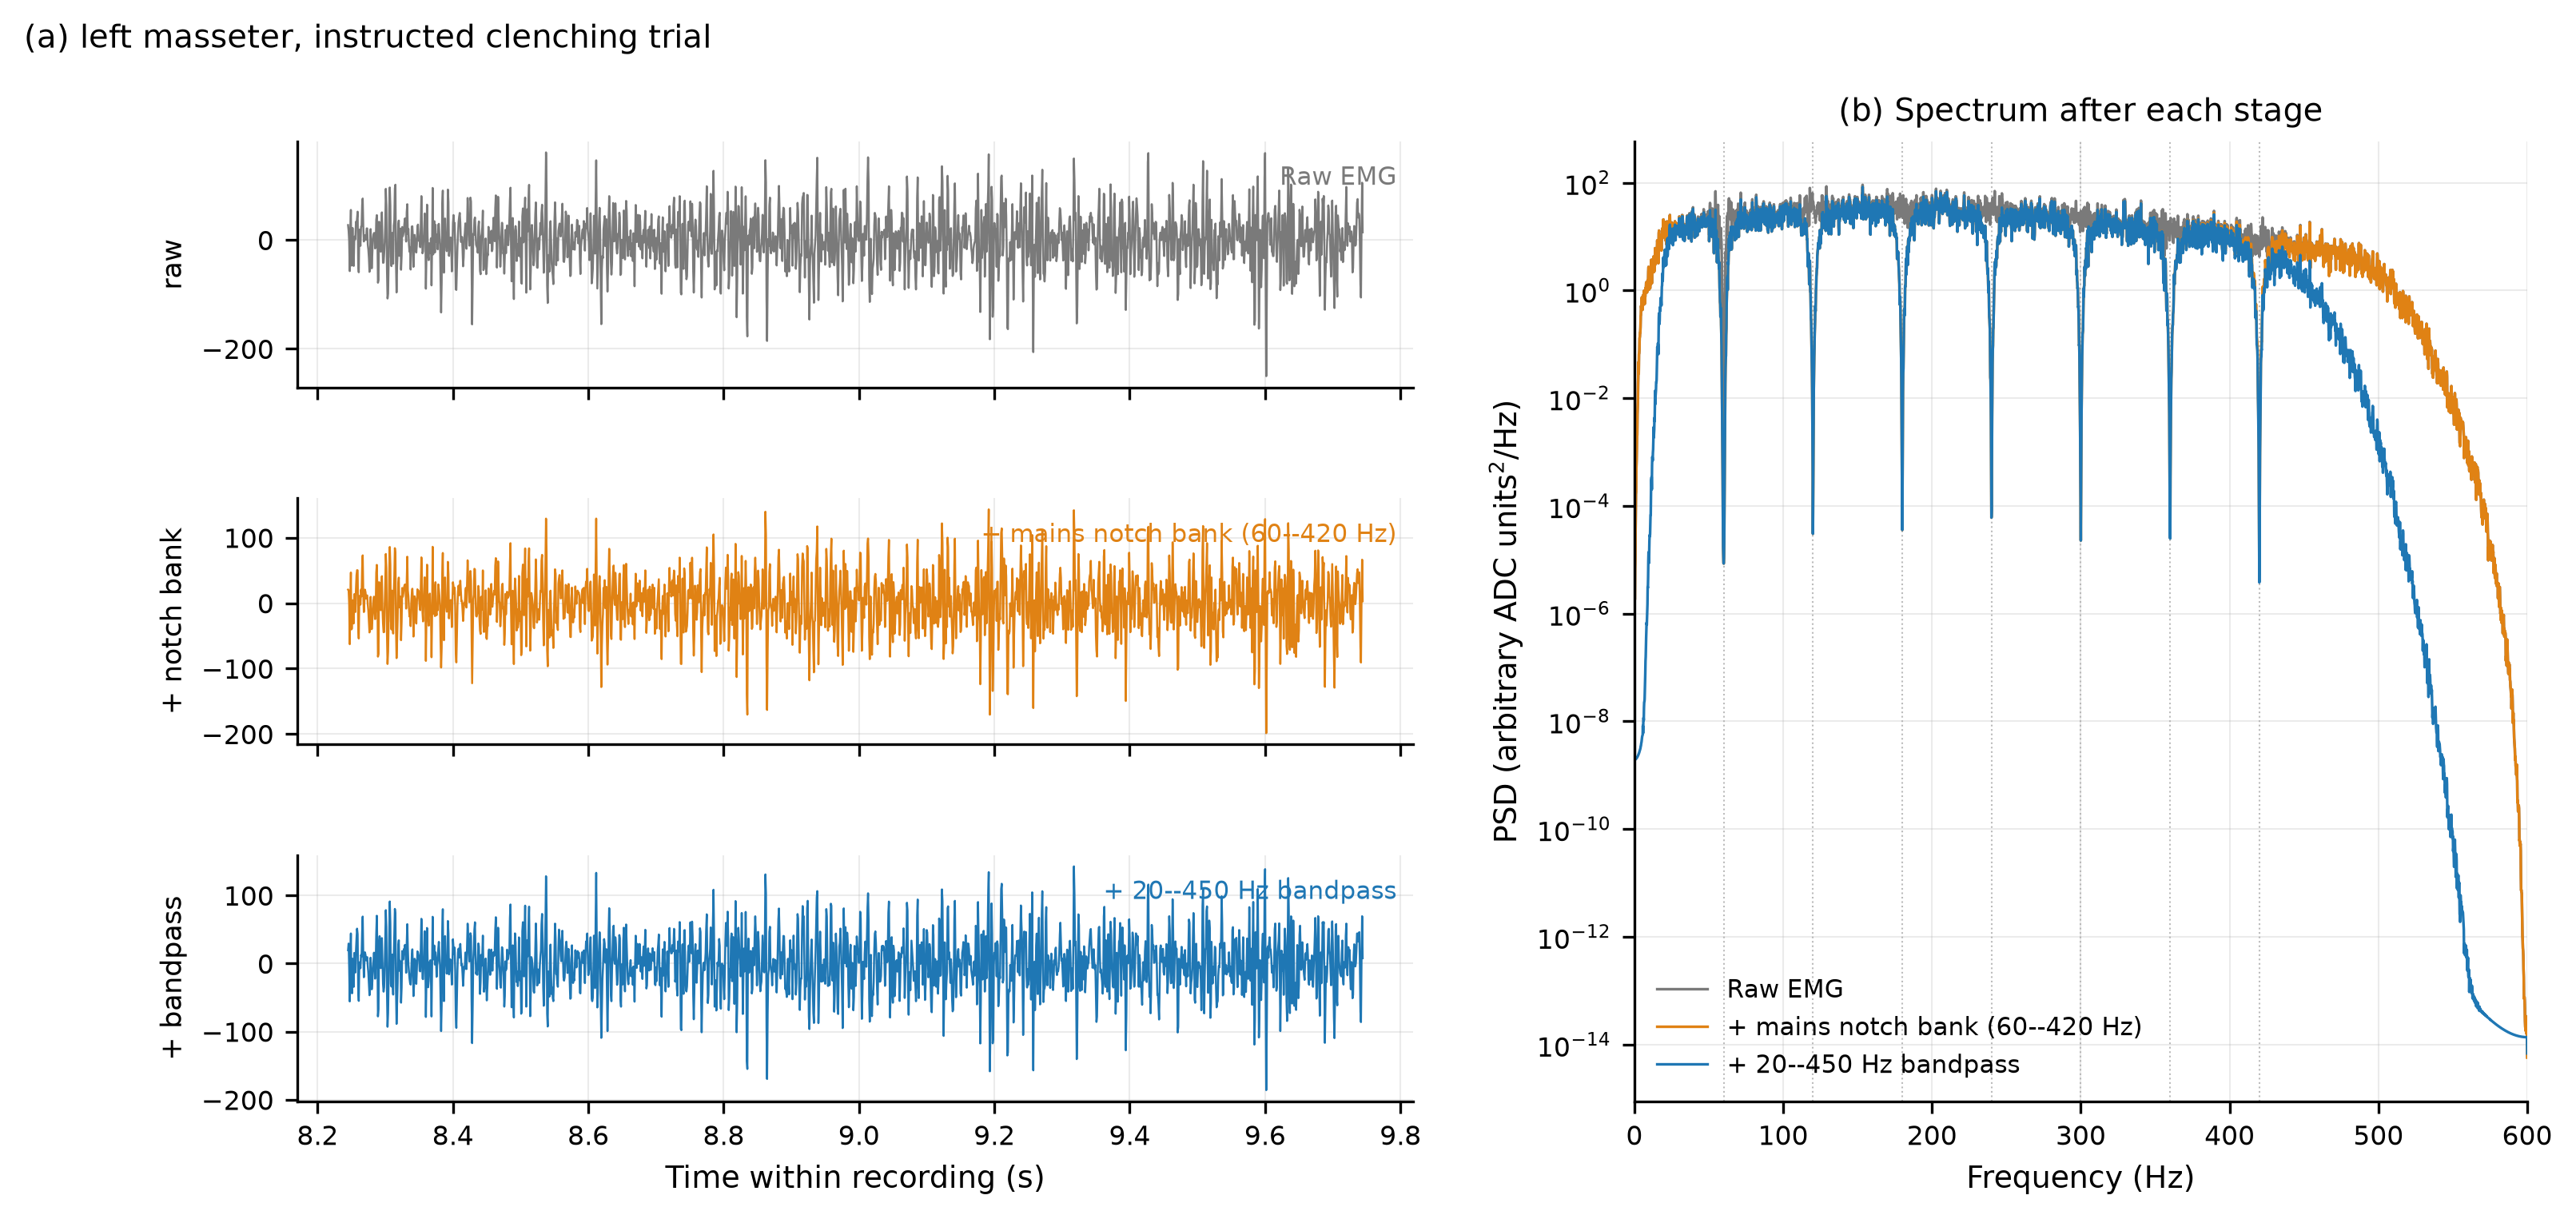
\includegraphics[width=0.76\linewidth]{Figures/preprocessing_stages_5class.png}
  \caption{Production preprocessing on a real excerpt of an instructed clenching trial (left masseter channel). (a) Time domain and (b) power spectrum after each stage: the notch bank removes the seven mains multiples marked by dotted lines, and the band-pass then removes content outside 20--450~Hz. The chain is applied to the continuous recording; windows are cut afterwards.}
  \label{fig:preprocessing}
\end{figure*}

\begin{figure*}[t]
  \centering
  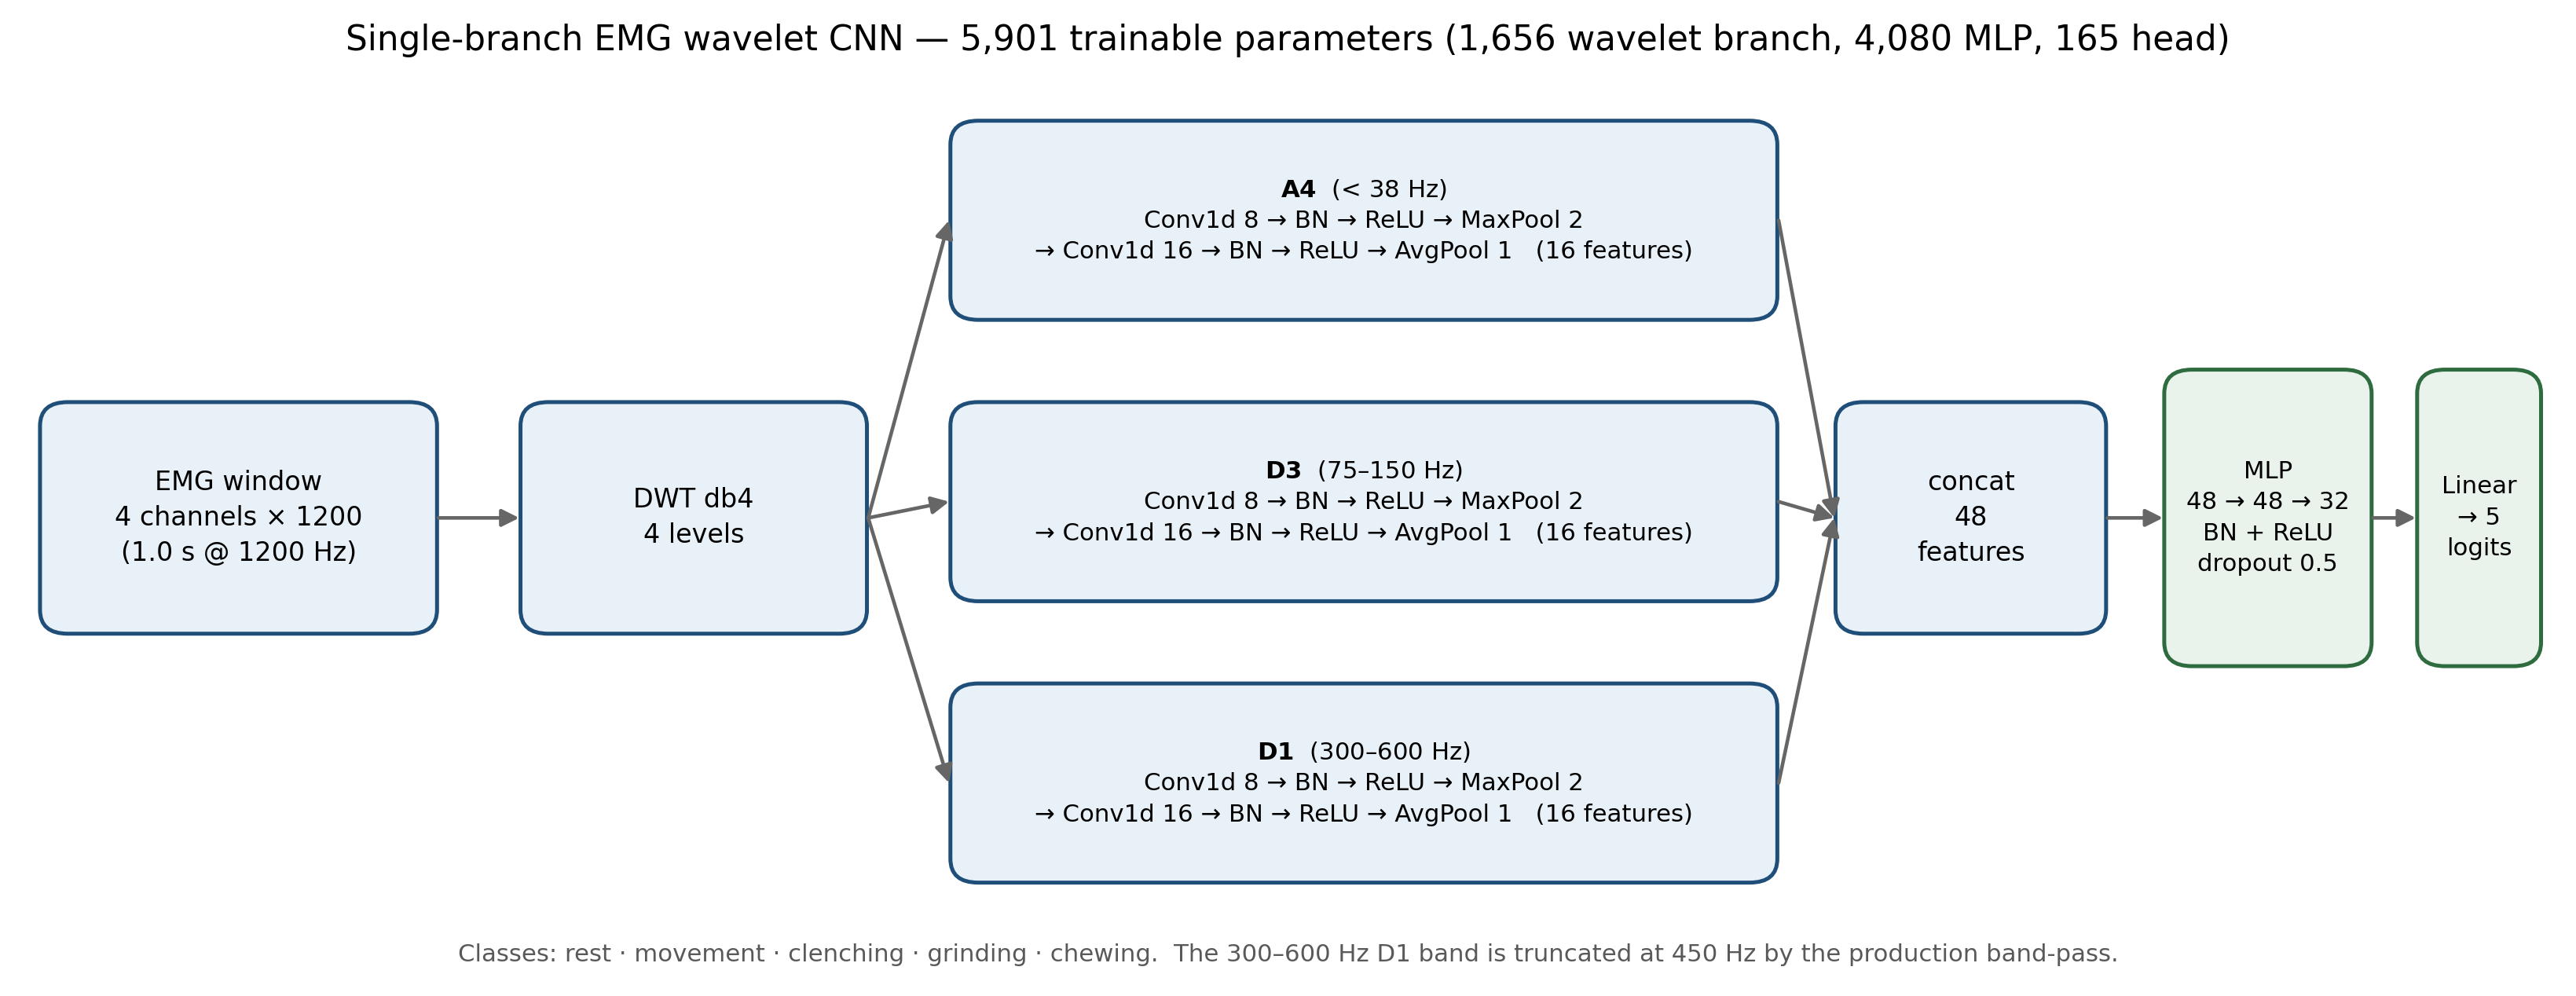
\includegraphics[width=0.84\linewidth]{Figures/v5/architecture_emg.png}
  \caption{Single-branch wavelet CNN. The four EMG channels undergo a db4 decomposition; three retained bands pass through parallel per-band CNN sub-branches, are concatenated, and are classified by an MLP with outputs for the five classes. Layer widths, wavelet family, band edges and parameter counts are read from the instantiated model rather than transcribed.}
  \label{fig:architecture}
\end{figure*}

\subsection{Training and evaluation}
\label{sec:training}

Class imbalance was addressed with inverse-frequency class weights recomputed within each outer training fold, and with augmentation of minority-class training windows by amplitude scaling in $[0.9, 1.1]$ (probability 0.5), additive Gaussian noise at 2\% of the window standard deviation (probability 0.3) and circular shifts of up to $\pm50$ samples (probability 0.3). A window was eligible with probability 0.4 and only if its class fell below 70\% of the largest class in that fold, so chewing windows were never augmented and rest windows were. Augmentation is confined to the training partition structurally: the augmenter raises an error for any other stage, and each transformation is seeded by the triple (run seed, epoch, sample identifier) so it does not depend on worker count or batch order. Optimisation used AdamW~\cite{loshchilov2019decoupled} and focal loss~\cite{lin2017focal} in PyTorch~\cite{paszke2019pytorch}, with the settings in Table~\ref{tab:hyperparameters}; the loss and learning rate were fixed rather than searched, so that no condition could win by drawing a better hyperparameter.

Evaluation used \emph{nested} LOSO, because selecting a model and reporting its score on the same held-out data biases the estimate upward~\cite{cawley2010overfitting,varma2006bias}. In each of the five outer folds one participant was sealed as the test set and the remaining four entered a participant-grouped inner LOSO loop of four folds; every normalisation statistic, class weight and augmentation minority set was fitted on inner-training participants only. The best epoch was recorded per inner fold by validation macro-F1, and the model was refit on all four outer-training participants for the median of those best epochs---no early stopping, no validation set---before the held-out participant was evaluated exactly once. That participant's sample identifiers are stored privately and released only by an explicit single-use call, so selection code cannot reach them even accidentally. Macro-F1 was the selection objective rather than accuracy, because accuracy is dominated by chewing~\cite{chicco2020advantages}. Three seeds all completed all five outer folds; metrics are computed independently per seed and then summarised, probabilities are never averaged across seeds and no seed is selected as best. Across the fifteen fold--seed combinations the epoch budget ranged from 15 to 43 (median 19), and the five-class conditions took 1.1~h of the 4.8~h the complete matched run required.

\textbf{Participant-level metrics are primary.} Accuracy, balanced accuracy, macro precision, recall, F1 and one-vs-rest ROC--AUC are computed within each held-out participant and then summarised across the five, with all five individual values reported. Pooled-window metrics are descriptive only, because windows within a participant and recording are correlated. AUC was computed from saved held-out probabilities, never from hard labels or a confusion matrix, and a class absent from a fold receives no AUC rather than an imputed value. No window-level bootstrap intervals or $p$-values are reported: the windows are clustered and overlapping, and with five participants such tests would overstate precision without supporting a population-level claim~\cite{lehmann2006testing,demsar2006statistical}. Held-out probabilities are uncalibrated (expected calibration error 0.063) and must not be read as probabilities~\cite{guo2017calibration}, though every AUC remains valid because AUC is rank-based and unaffected by monotone rescaling.

Two secondary analyses were computed post hoc from the same held-out five-class predictions and are labelled as such: chewing windows removed and the remaining four probabilities renormalised, with a separately trained four-class model run on the same windows and folds as a check that renormalisation is not doing the work; and predictions collapsed into instructed clenching/grinding versus rest/movement/chewing. Both re-read one model rather than training a new one, and the second is task discrimination, not bruxism detection, because the positive tasks were elicited and the background class excludes unrestricted free-living behaviour.

\subsection{Feature baselines and the screening harness}
\label{sec:screening}

Two families of measurement come from a deliberately cheap \emph{screening} harness rather than the confirmatory protocol, and every value it produces is labelled as such. The harness extracts 28 hand-written features per window---per EMG channel, the log RMS of each of five db4 bands, the log waveform length and the zero-crossing rate~\cite{phinyomark2012feature}---and fits one model per outer fold with no nested hyperparameter selection, using multinomial logistic regression and histogram gradient boosting~\cite{pedregosa2011scikit}. Because the feature set was chosen after looking at these five participants and no nested selection is performed, screening numbers are directionally reliable and optimistic in level; they decide which change is worth a confirmatory run and are never reported as a result. The harness supplies the matched before-and-after comparison for RQ1 (Section~\ref{sec:rq1}) and the hand-engineered baseline for RQ3 (Section~\ref{sec:rq3})---the relevant comparison for a network whose per-band sub-branches reduce each band to a pooled amplitude, since a learned representation that cannot beat the band energies it is built from is not earning its place. Both run on the identical 6,173 windows and five outer folds as the confirmatory model.

\begin{table}[t]
  \caption{Training and evaluation configuration. The loss and learning rate were fixed rather than searched, so that the conditions of the same run differ only in what they were asked to do.}
  \label{tab:hyperparameters}
  \centering
  \footnotesize
  \begin{tabular*}{\columnwidth}{@{\extracolsep{\fill}}ll@{}}
    \toprule
    Hyperparameter & Value \\
    \midrule
    Optimiser & AdamW \\
    Learn.\ rate / weight decay & $10^{-3}$ / $10^{-4}$ \\
    Loss & Focal, $\gamma = 1.5$ \\
    Class weights & Inverse freq., per fold \\
    Dropout / batch size & 0.5 / 64 \\
    Gradient clipping & Norm 1.0 \\
    Epoch budget & Median inner best (15--43) \\
    Seeds & 0, 1, 2 \\
    Outer / inner folds & 5 / 4, ppt-grouped \\
    Normalisation scope & Strict (outer-train ppts) \\
    \bottomrule
  \end{tabular*}
\end{table}

\subsection{The channel that is not analysed}
\label{sec:mic}

An omnidirectional microphone was secured near the temporomandibular joint (Fig.~\ref{fig:setup}a) and recorded alongside the electromyogram to support offline annotation: an experimenter reviewing a trial can hear when tooth contact occurs. No result in this paper reads it, and the exclusion rests on measurements rather than preference, so that it can be checked.

First, the channel is not an acoustic waveform. It is integer-valued with a quantisation step of exactly 1 count over a range of roughly 50--227, and 96\% of its power lies below 10~Hz (range 91.4--98.7\%), concentrated at the 1--3-Hz masticatory rhythm, so it behaves as a rectified sound-level output; at the 1200-Hz acquisition rate the 600-Hz Nyquist frequency also sits below the band in which tooth contact radiates most of its energy~\cite{romano2024wearable}. Second, it is not synchronous with the electromyogram: over the 45 chewing recordings, where every muscle burst coincides with an impact, the envelope cross-correlation at zero lag has a median of $-0.017$ and peaks at a median absolute lag of 18~s. Third, and decisively, a rotation-invariant fingerprint of every channel of every recording shows 100 distinct waveforms on each EMG channel but only 37 on the microphone channel: 83 of the 100 recordings carry a microphone waveform bit-identical, after a circular rotation, to another \emph{participant's} recording of the same condition. A LOSO protocol therefore never holds that channel out, and no second copy exists to recover---the three surviving \texttt{.npy} acquisition companions reproduce the electromyographic and trigger columns exactly but carry an all-zero microphone column, and the video files have no audio stream.

A matched modality ablation had already been run on this channel before the fingerprinting audit, under the protocol of Section~\ref{sec:training} and on the same windows, folds and seeds as everything else reported here. Adding the microphone branch changed participant-level macro-F1 by $+0.009$ on the five-class task and $+0.004$ with chewing removed, both smaller than the spread between seeds, and the microphone alone reached 42.8\% macro-F1 against 72.0\% for EMG alone. Those figures are consistent with a channel that contributes almost nothing, but the duplication means they cannot be quoted as a measurement of what a microphone contributes. The defensible statement is the negative one: this channel was not usable, EMG carries the classification on its own, and whether a working transducer would help is untested rather than answered (Section~\ref{sec:mic_discussion}). The exclusion is now enforced rather than remembered: the pipeline fingerprints every channel of every recording, groups them, and refuses any run whose held-out participant's signal appears in its own training set, at a cost of one pass over the data.

\section{Results}

The confirmatory results come from the EMG conditions of one nested-LOSO run on the corrected signal: five outer folds $\times$ three seeds, 6,173 held-out window predictions per seed, 18,519 in total for the five-class task and a further 7,614 for the separately trained four-class task. Every value was recomputed from the saved prediction ledgers, in which each held-out window appears exactly once per task, model and seed. Screening values are marked wherever they appear.

\subsection{RQ1: what the measurement chain contributes}
\label{sec:rq1}

The filter chain was changed while the windows, folds and labels were held identical, so the comparison isolates the chain (Table~\ref{tab:filter}, Fig.~\ref{fig:measurement_chain}). Identical is meant literally: the 6,173 windows, their five outer-fold assignments and their class labels are the same objects in both arms, verified by comparing the two prediction ledgers window by window.

The confirmatory network answers the question directly. Through the superseded chain it reached 55.0\% accuracy, 43.5\% participant-level macro-F1 and a macro one-vs-rest AUC of 0.785; through the corrected chain the matched condition reached 80.9\%, 72.8\% and 0.963---a gain of 29.3 points of macro-F1, 25.9 of accuracy and 0.178 of AUC---and the share of quiet-rest windows misread as clenching or grinding fell from 30.2\% to 6.1\%. The contrast is conservative twice over: the superseded run also searched the loss and learning rate inside each fold, which the corrected run fixed, and both arms are the fused condition, so the superseded arm carried an input channel it could exploit. The corrected EMG-only condition reported throughout the rest of this paper scores 72.0\% macro-F1, within a point of its fused counterpart.

The screening harness reproduces the effect with two much simpler estimators, which rules out an idiosyncrasy of the network: logistic regression on the 28 EMG band-energy features moved from 53.1\% accuracy and 37.3\% macro-F1 to 78.3\% and 63.9\%, and gradient boosting from 38.8\% to 61.3\% macro-F1. Three estimators of very different capacity move by 22 to 29 points, and none saw a new window, a new label or a new fold. The per-participant view shows how severe the earlier state was: through the superseded chain two of the five held-out participants were essentially unclassifiable---P1 at 18.1\% macro-F1 and 26.9\% accuracy, P2 at 5.4\% and 6.9\%, both at or below what a constant prediction would achieve---while P3--P5 scored 57.6--75.4\%; after the correction the same five span 61.4--82.4\%. What had looked like severe between-participant heterogeneity, the standard reading of such a spread and the one that motivates transfer learning and per-user calibration, was substantially an artifact of interference differing between recording sessions.

Three further measurements establish that the superseded chain was not merely suboptimal but inert, and explain the mechanism. First, the 60-Hz notch was doing nothing: a control chain with \emph{no} mains removal at all---band-pass only---scored 38.5\% macro-F1, within 1.2 points of the superseded chain's 37.3\% and comfortably inside the range of the two. Filtering the fundamental the hardware had already removed was, to the precision this comparison can resolve, equivalent to not filtering. Second, the interference was large enough to be the dominant signal. Expressed as each activity's median RMS divided by \emph{that participant's own} resting RMS---the contrast a classifier must exploit---the superseded chain left chewing at 1.6--7.2$\times$ rest and clenching at 1.6--5.2$\times$; after correction the same quantities are 8.5--35.7$\times$ and 8.1--27.0$\times$ (Fig.~\ref{fig:measurement_chain}c). The physiological contrast was present the whole time, buried under interference that varied more between people than the physiology varied between conditions. Third, that is what the between-participant statistics show: the superseded chain left a $5.07\times$ spread between the largest and smallest participant median RMS and 20 pairs in which one person's \emph{resting} EMG exceeded another's \emph{active} EMG, against $2.97\times$ and no such pairs after correction (Fig.~\ref{fig:measurement_chain}d). A model trained on the earlier signal could reduce its loss by learning which participant a window came from rather than what that participant was doing, and LOSO is the protocol that then reports the consequence as poor generalisation. The screening arm shows the same per-participant pattern (Fig.~\ref{fig:measurement_chain}b): P2, who gained most, moved from 0.135---below the 0.165 a uniform guess would score---to 0.645.

\begin{table*}[t]
  \centering
  \caption{RQ1. The EMG filter chain is the only thing that varies: the same 6,173 windows, the same five outer-fold assignments and the same labels in every arm, verified window by window across the two prediction ledgers. Residual mains power is the share of 20--450-Hz power within $\pm3$~Hz of a mains multiple, averaged over participant $\times$ class cells; a perfectly white signal would score 0.098. ``Inv.'' counts participant pairs in which one person's resting EMG exceeded another person's active EMG. Differences quoted in the text are computed before rounding.}
  \label{tab:filter}
  \footnotesize
  \begin{tabular*}{\textwidth}{@{\extracolsep{\fill}}lcccccc@{}}
    \toprule
    & \multicolumn{3}{c}{Measured signal properties} & \multicolumn{3}{c}{Participant-level macro F1} \\
    \cmidrule(lr){2-4}\cmidrule(lr){5-7}
    EMG chain & \shortstack{Residual\\mains} & \shortstack{Ampl.\\spread} & Inv. & \shortstack{Wavelet\\CNN$^{a}$} & \shortstack{Logistic\\reg.$^{b}$} & \shortstack{Grad.\\boost.$^{b}$} \\
    \midrule
    60 Hz notch only (superseded) & 0.673 & $5.07\times$ & 20 & 43.5\% & 37.3\% & 38.8\% \\
    Band-pass only (control) & 0.671 & $5.02\times$ & 20 & --- & 38.5\% & 39.2\% \\
    \midrule
    \textbf{Mains notch bank, 8 Hz (used)} & \textbf{0.012} & $\mathbf{2.97\times}$ & \textbf{0} & \textbf{72.8\%} & \textbf{63.9\%} & \textbf{61.3\%} \\
    \bottomrule
  \end{tabular*}
  \begin{flushleft}\footnotesize
  The notch bank was selected on residual mains power, a criterion specifiable in advance, not on classification score. A constant-$Q$ bank at the identical 13\% band cost scored marginally higher in screening (0.689 against 0.679 macro-F1 on the full 35-feature set) while leaving eight times the residual interference, and would have been selected by a score criterion.\\
  $^{a}$Confirmatory nested LOSO, three seeds, five outer folds. Both rows are the fused condition, so the two are like-for-like on modality; the superseded row additionally searched the loss and learning rate inside each fold, which the corrected row fixed, so the comparison favours the superseded arm on both counts. The corrected EMG-only condition reported elsewhere in this paper scores 72.0\%.\\
  $^{b}$Screening harness on the 28 EMG features: one fit per outer fold, no nested selection, feature set chosen after seeing these participants. Optimistic in level; reported here for the contrast and to show that it does not depend on model capacity.
  \end{flushleft}
\end{table*}

\begin{figure*}[t]
  \centering
  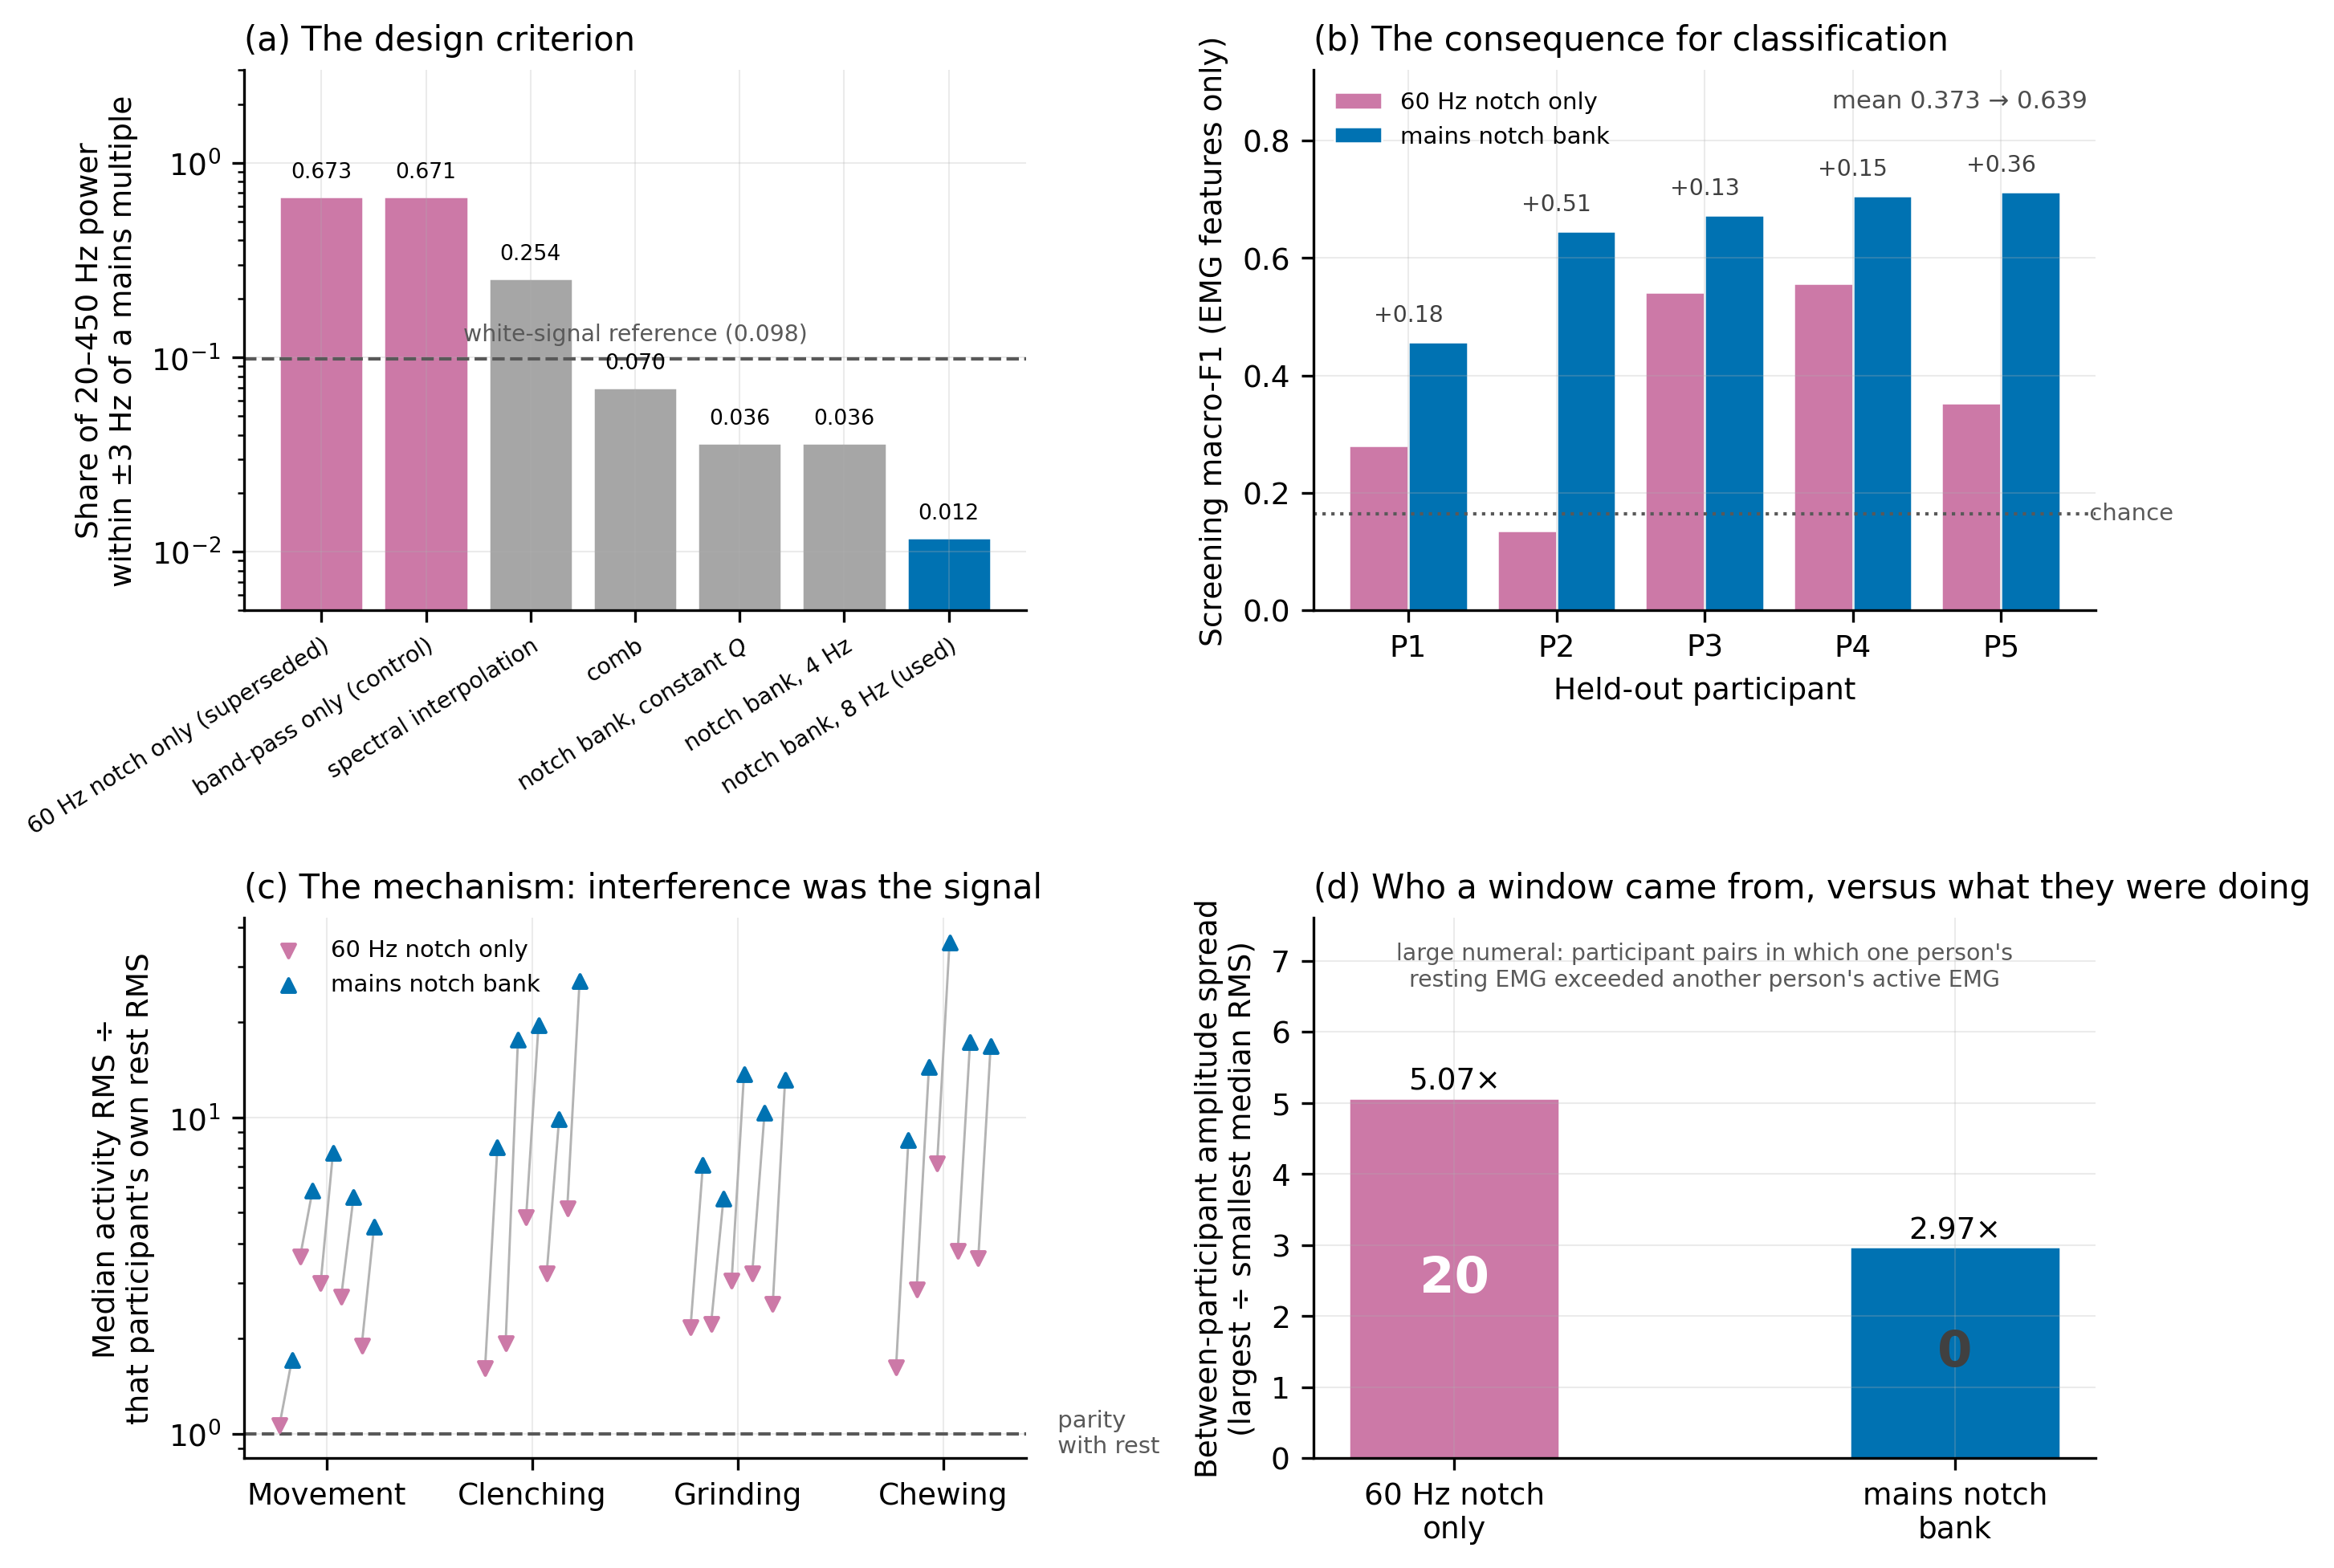
\includegraphics[width=0.76\linewidth]{Figures/v5/measurement_chain.png}
  \caption{The mains-harmonic defect, in the terms a classification paper is read in. (a) Residual mains power for every candidate chain implemented and measured, against the 0.098 a white signal would score; the chain used is the lowest, and was chosen on this axis rather than on classification score. (b) Screening macro-F1 per held-out participant before and after the correction, on the 28 EMG features and identical folds. (c) The mechanism: each activity's median RMS divided by that participant's own resting RMS, five participants per condition, before (down triangles) and after (up triangles). (d) Between-participant amplitude spread, and the number of pairs in which one person's resting EMG exceeded another's active EMG. No panel reads the microphone.}
  \label{fig:measurement_chain}
\end{figure*}

\subsection{RQ2: five-class performance on the corrected signal}

Averaged over the five held-out participants and three seeds, the model achieved 81.7\% accuracy, 77.6\% balanced accuracy, 72.0\% macro-F1 and a macro one-vs-rest ROC--AUC of 0.958 (Table~\ref{tab:results}). Seed-to-seed variation was small relative to variation between participants: accuracy 83.4\%, 81.5\% and 80.2\%; macro-F1 74.5\%, 69.9\% and 71.4\%; macro AUC 0.963, 0.953 and 0.957. Pooling held-out windows across participants---a descriptive summary only, because the windows are correlated---gives 80.7\% accuracy and 71.5\% macro-F1 at a macro AUC of 0.948.

Quiet rest reached 77.1\% precision, 91.4\% recall, an F1 of 83.6\% and a one-vs-rest AUC of 0.958: the second-best-separated class after chewing and the best-recalled of the five, which is the outcome the class was added to test. Activity windows can be scored against a quiet non-event condition rather than only against one another.

Per-class ROC and precision--recall curves are shown in Fig.~\ref{fig:roc_pr}. The class ordering is consistent across both views, but the two disagree sharply about the small classes, and the disagreement is informative: for the seed drawn, movement combines an AUC of 0.949 with an average precision of 0.615 and instructed grinding an AUC of 0.921 with an average precision of 0.597, while chewing at 58.9\% prevalence reaches 0.991 and 0.993. Precision--recall is sensitive to the very unequal class sizes and ROC is not~\cite{saito2015precision,davis2006relationship}, so a reader who sees only the AUC column of Table~\ref{tab:results} will overestimate how usable the minority classes are.

\begin{table*}[t]
  \centering
  \caption{Five-class performance on the corrected signal. The upper block gives participant-level means---computed within each held-out participant, then averaged over the five---so its rows are directly comparable; the lower block gives per-class values on pooled held-out windows, averaged over three seeds, with one-vs-rest AUC computed from held-out probabilities. Values describe this five-participant dataset and are not population-level superiority tests.}
  \label{tab:results}
  \small
  \begin{tabular*}{\textwidth}{@{\extracolsep{\fill}}lcccccc@{}}
    \toprule
    Method / class & Accuracy & Precision & Recall & F1 & AUC & Windows \\
    \midrule
    \multicolumn{7}{l}{\emph{Participant-level means, five held-out participants $\times$ three seeds}}\\
    \textbf{Wavelet CNN, 4-channel EMG} & \textbf{81.7\%} & \textbf{73.7\%} & \textbf{77.6\%} & \textbf{72.0\%} & \textbf{0.958} & 6,173 \\
    Logistic regression, band energies$^{a}$ & 78.3\% & -- & -- & 63.9\% & 0.965 & 6,173 \\
    Gradient boosting, band energies$^{a}$ & 74.8\% & -- & -- & 61.3\% & 0.914 & 6,173 \\
    \midrule
    \multicolumn{7}{l}{\emph{Wavelet CNN, per class, pooled held-out windows}}\\
    Rest & -- & 77.1\% & 91.4\% & 83.6\% & 0.958 & 590 \\
    Movement & -- & 34.4\% & 69.8\% & 46.0\% & 0.937 & 333 \\
    Clenching & -- & 70.5\% & 66.0\% & 68.1\% & 0.936 & 799 \\
    Grinding & -- & 67.9\% & 69.5\% & 68.6\% & 0.928 & 816 \\
    Chewing & -- & 97.3\% & 85.8\% & 91.1\% & 0.981 & 3,635 \\
    Macro average & 80.7\% & 69.4\% & 76.5\% & 71.5\% & 0.948 & 6,173 \\
    \bottomrule
  \end{tabular*}
  \begin{flushleft}\footnotesize
  Pooled-window macro AUCs are 0.948 for the CNN, 0.944 for logistic regression and 0.894 for gradient boosting.\\
  $^{a}$Screening harness (Section~\ref{sec:screening}): one model fit per outer fold, no nested hyperparameter selection, feature set chosen after seeing these participants. Optimistic in level, which makes the network's margin over these rows a conservative estimate. Macro precision and recall are not reported for these rows because the harness stores a prediction ledger rather than a per-class table.
  \end{flushleft}
\end{table*}

\begin{figure*}[t]
  \centering
  
\includegraphics[width=0.41\linewidth]{Figures/v5/five_class_roc_curves.png}
  \hfill
  
\includegraphics[width=0.41\linewidth]{Figures/v5/five_class_pr_curves.png}
  \caption{One-vs-rest ROC (left) and precision--recall (right) curves for the five classes, pooled over the held-out windows of seed 0 (the lowest seed index, a fixed rule rather than a post-hoc choice). Each curve depicts one trained model per fold, so legend values are that seed's; three-seed means are in Table~\ref{tab:results}. Precision--recall separates the classes far more sharply than ROC, because it is sensitive to the very unequal class sizes.}
  \label{fig:roc_pr}
\end{figure*}

\subsection{Class-level and participant-level behaviour}
\label{sec:diagnostics}

The highest per-class F1 was chewing's (91.1\%), the lowest movement's (46.0\%). Movement's is a precision problem rather than a detection problem: recall 69.8\% and AUC 0.937, but precision 34.4\%, because it is the smallest class (333 windows, 5.4\% of the total) and absorbs 9.9\% of the eleven-times-more-numerous chewing windows. Clenching and grinding are the hardest pair to separate---19.5\% of clenching windows were labelled grinding and 14.5\% of grinding windows clenching, together the majority of both classes' errors. Rest had the highest recall of any class at 91.4\%, and its dominant error was into grinding (7.5\%, against 0.3\% into clenching), so confusion between quiet rest and the combined clenching/grinding group occurred in 7.7\% of rest windows---the errors that carry most weight, because they approximate false alarms under the limited quiet-rest condition. For the seed in Fig.~\ref{fig:diagnostics}a the diagonal counts were 534 of 590 rest windows, 242 of 333 movement, 542 of 799 clenching, 589 of 816 grinding and 3,187 of 3,635 chewing.

Table~\ref{tab:persubject} reports five-class results for each held-out participant and Fig.~\ref{fig:diagnostics}b shows the same values with their individual seeds. Accuracy ranged from 73.4\% to 90.7\%, macro-F1 from 63.2\% to 80.5\% and macro AUC from 0.904 to 0.981; the spread is substantial relative to the mean and is not explained by class balance alone. Two participants show why accuracy and AUC must be read together. P4 had the lowest accuracy alongside the second-highest AUC (74.0\% and 0.981): its windows are ranked well, and the loss is concentrated in where the decision boundaries fall rather than in the ability to order windows. P1 shows the opposite---the lowest AUC (0.904) and macro-F1 (63.2\%) at an accuracy no better than P4's---and contributes the largest single share of windows (1,692 of 6,173), so it dominates any pooled-window summary while counting as one of five at participant level. That is one concrete reason participant-level aggregation is primary here. With five participants the tabulated standard deviations describe the sample rather than a sampling distribution, and no population-level estimate follows from the mean.

t-distributed stochastic neighbour embedding (t-SNE)~\cite{vandermaaten2008visualizing} of the 32-dimensional penultimate representation (Fig.~\ref{fig:tsne}) reproduces both error patterns: chewing occupies several large, well-separated regions, consistent with its high AUC and food-dependent rhythmic structure; rest forms tight compact islands, as a low-variance quiet condition should; clenching and instructed grinding share adjacent, partly interleaved territory; and movement scatters along the borders of the larger classes. t-SNE distances are not metric, so the embedding is corroboration only.

\begin{figure*}[t]
  \centering
  
\includegraphics[width=0.49\linewidth]{Figures/v5/confmatrx_5class.png}
  \hfill
  
\includegraphics[width=0.39\linewidth]{Figures/v5/five_class_per_participant.png}
  \caption{Held-out behaviour of the reported model. (a) Confusion matrix pooled across the five LOSO folds of seed 0 (fixed lowest-seed-index rule, not selected by score), as counts and row-normalised recall. The dominant error patterns are the mutual clenching--grinding confusion and the leakage of chewing windows into the much smaller movement class. (b) Macro-F1 per held-out participant: bars are the mean over three seeds, open markers the individual seeds, and the label inside each bar that participant's held-out window count. Five participants cannot characterise population variability, so no generalisation claim follows from the mean.}
  \label{fig:diagnostics}
\end{figure*}

\begin{table}[t]
  \caption{Five-class performance for each held-out participant, averaged over three seeds.}
  \label{tab:persubject}
  \centering
  \footnotesize
  \begin{tabular*}{\columnwidth}{@{\extracolsep{\fill}}lrrrr@{}}
    \toprule
    Held out & $n$ & Acc. & Macro F1 & Macro AUC \\
    \midrule
    Participant 1 & 1,692 & 73.4\% & 63.2\% & 0.904 \\
    Participant 2 & 1,007 & 90.7\% & 72.6\% & 0.957 \\
    Participant 3 & 1,133 & 83.7\% & 71.3\% & 0.967 \\
    Participant 4 & 1,167 & 74.0\% & 72.2\% & 0.981 \\
    Participant 5 & 1,174 & 86.7\% & 80.5\% & 0.980 \\
    \midrule
    Mean & 6,173 & 81.7\% & 72.0\% & 0.958 \\
    SD & --- & 7.7 & 6.1 & 0.032 \\
    \bottomrule
  \end{tabular*}
\end{table}

\begin{figure}[t]
  \centering
  
\includegraphics[width=0.92\linewidth]{Figures/v5/tsne_5class.png}
  \caption{t-SNE of the 32-dimensional learned penultimate representation for held-out windows, coloured by experimental class. Embeddings were recomputed from the saved fold checkpoints using only outer-test windows of one seed, so each held-out window appears exactly once.}
  \label{fig:tsne}
\end{figure}

\subsection{Secondary analyses with rest}
\label{sec:secondary}

Excluding chewing leaves a four-class problem over rest, movement, clenching and grinding, which yielded 77.7\% accuracy, 75.7\% macro-F1 and a macro AUC of 0.942 at participant level, and 75.4\%, 75.4\% and 0.919 on pooled windows (Table~\ref{tab:sensitivity}). Removing chewing lowers accuracy by 4.0 points but \emph{raises} macro-F1 by 3.7, because the metric is no longer dominated by a single large, easily separated class. A model trained separately on the same four classes reaches 77.7\% accuracy, 75.8\% macro-F1 and 0.942 AUC---agreement to within a tenth of a point on macro-F1, confirming that the post-hoc values are not an artifact of renormalisation.

Treating clenching and grinding as the positive group and rest, movement and chewing as the comparison group yielded 92.5\% accuracy, 86.4\% precision, 84.8\% sensitivity, 95.3\% specificity, an F1 of 85.5\% and an AUC of 0.970 on pooled windows, and 93.0\% accuracy with a participant-level macro-F1 of 89.3\% and AUC of 0.968. Within the quiet-rest condition, 7.7\% of rest windows (45, 50 and 42 of 590 across the three seeds) fell on the tooth-contact side. This analysis includes a laboratory non-event class but does not measure detection in a continuous free-living stream: a 7.7\% per-window false-alarm rate at a 0.5-s decision interval corresponds to roughly 550 false alarms per hour if the background were quiet rest throughout---the quantity a deployable detector must report, and one this design cannot estimate.

\begin{table*}[t]
  \caption{Secondary analyses computed post hoc from the held-out five-class predictions, averaged over three seeds. These re-read one trained model; they are not separately trained tasks.}
  \label{tab:sensitivity}
  \centering
  \small
  \begin{tabular*}{\textwidth}{@{\extracolsep{\fill}}lcccccc@{}}
    \toprule
    Analysis & Accuracy & Precision & Recall & Specificity & F1 & AUC \\
    \midrule
    Excluding chewing$^{a}$ & 75.4\% & 74.9\% & 76.1\% & -- & 75.4\% & 0.919 \\
    Collapsed binary$^{b}$ & 92.5\% & 86.4\% & 84.8\% & 95.3\% & 85.5\% & 0.970 \\
    \bottomrule
  \end{tabular*}
  \begin{flushleft}\footnotesize
  Values are pooled over held-out windows. The corresponding participant-level means are 77.7\% accuracy / 75.7\% macro-F1 / 0.942 AUC when chewing is excluded, and 93.0\% / 89.3\% / 0.968 for the collapsed binary analysis.\\
  $^{a}$Macro precision, recall, F1 and one-vs-rest AUC across rest, movement, clenching and grinding, after removing chewing windows and renormalising the remaining four probabilities. A separately trained four-class model on the same windows and folds reaches 77.7\% accuracy and 75.8\% participant-level macro-F1.\\
  $^{b}$Instructed clenching/grinding treated as positive; rest/movement/chewing treated as the comparison group. This is task discrimination, not clinical diagnosis.
  \end{flushleft}
\end{table*}

\subsection{RQ3: the learned representation against its alternatives}
\label{sec:rq3}

On the identical 6,173 windows and five outer folds, the screening harness reached 63.9\% macro-F1 at 78.3\% accuracy with logistic regression on 28 EMG band-energy features, and 61.3\% at 74.8\% with gradient boosting (Table~\ref{tab:results}). Every value is a participant-level mean computed exactly as the network's are. The network's 72.0\% macro-F1 exceeds these by 8.1 and 10.6 points and its accuracy by 3.4 and 6.9; because the harness fits one model per fold with a feature set chosen after seeing these participants, the margin over it is a conservative estimate, and the direction is stable across two very different estimators.

The AUC column does not follow, and the discrepancy is worth stating rather than omitting. Logistic regression reaches a participant-level macro AUC of 0.965 against the network's 0.958, and on pooled windows the ordering reverses, 0.944 against 0.948. Both differences are smaller than the network's own seed-to-seed AUC range (0.953--0.963), so the two models rank held-out windows about equally well and the network's advantage lies in where its decision boundaries fall once those windows are ranked. That is the same dissociation between ranking and thresholding that separates P1 and P4 in Section~\ref{sec:diagnostics}, and it is why macro-F1 rather than AUC was the prespecified selection objective.

One qualification matters more than the margin: the advantage was much smaller before the measurement chain was corrected. Through the superseded chain, on the identical windows and folds, the network reached 43.5\% macro-F1 against 39.3\% for logistic regression and 40.1\% for gradient boosting on the 35-feature screening set---a margin of 4.2 and 3.5 points, obtained by a network that additionally searched its loss and learning rate and additionally carried a microphone branch matched by seven of the baselines' features. That near-parity had been read at the time as evidence that the architecture contributed nothing over band energies. The reading was correct about the numbers and wrong about the cause. When the dominant variance in a window is interference amplitude, a per-band pooled amplitude is all there is to extract, and a network whose sub-branches compute pooled band amplitudes cannot beat features that compute them directly. Once the interference is removed the margin roughly doubles, against baselines that no longer read a second channel.

%%%% RQ3-DEEP-BASELINES --------------------------------------------------------------
%%%% Run baselines_emg_only_20260816 (configs/experiments/baselines_emg_only.yaml) is the
%%%% prespecified architecture sweep on the corrected chain: dual_branch_wavelet_cnn,
%%%% dual_branch_temporal_cnn, early_fusion_cnn, bilstm; all modality=emg_only; identical
%%%% windows, folds and seeds. Replace the subsection below with the measured comparison
%%%% and add a block to Table~\ref{tab:results} when it completes.
%%%% ----------------------------------------------------------------------------------

\subsection{Alternative learned architectures}
\label{sec:deep_baselines}

Band energies are not the only alternative. A prespecified sweep contrasts four architectures under one training configuration and identical inputs: the wavelet CNN above; a dual-branch temporal CNN that keeps the time axis, pools each band by mean, standard deviation and maximum rather than by mean alone, and adds a modulation-spectrum head so that burst--relaxation rhythm is representable at all; an early-fusion CNN on the raw signals; and a bidirectional LSTM. Every model receives the same four EMG channels on the same 6,173 windows, the same five outer folds and the same three seeds, because a table in which the proposed model receives one input set and the baselines another measures the inputs rather than the architecture. The earlier measurements of this sweep were taken through the defective chain and are superseded rather than reproducible; Table~\ref{tab:architectures} reports it on the corrected signal.

Two findings matter more than the ordering itself. First, the wavelet decomposition earns its place against raw signals. The early-fusion CNN reads the same four channels through 19,029 parameters---3.2 times the wavelet network's 5,901---and reaches 68.9\% macro-F1 against 72.2\%, while the bidirectional LSTM is worse again at 60.2\%. On these recordings, capacity applied to the raw waveform is no substitute for an explicit band decomposition.

Second, and against the model this paper otherwise reports, the dual-branch temporal CNN is the strongest of the four: 75.0\% macro-F1 at a macro AUC of 0.974, against 72.2\% and 0.954. The gap is small but consistent. Every one of its three seeds exceeds every one of the wavelet network's on macro-F1 (0.736--0.762 against 0.705--0.734), and the two AUC ranges do not overlap at all (0.971--0.976 against 0.948--0.958), so the ordering is not an artifact of which seeds were drawn. It is nevertheless bought with parameters---17,981 against 5,901, a threefold increase---and it is not uniform across participants: the temporal network gains 7.0 points of macro-F1 on P1, 6.6 on P3 and 7.5 on P5, but loses 6.7 on P2 and ties on P4. With five participants, a 2.8-point mean difference resting on three of them is a direction rather than an effect size.

What makes that direction worth reporting is its source rather than its size. The temporal network differs from the wavelet network in exactly two respects: it summarises each band by mean, standard deviation and maximum instead of the mean alone, and it carries a modulation-spectrum head, so a burst--relaxation rhythm at 1--2~Hz is representable inside a single window at all. That is precisely the information Section~\ref{sec:constraints} shows the 1.0-s window withholding, and prices there at 7.4 points of screening macro-F1. The ordering across all four models is therefore a statement about representation rather than capacity: the two largest networks in the table occupy its first and third places, separated by whether they see the signal in wavelet bands and whether they can see its rhythm.

\begin{table*}[t]
  \centering
  \caption{RQ3. Four architectures on identical inputs: the same 6,173 windows, the same five outer folds and the same three seeds, every model reading the same four EMG channels under one fixed training configuration. Values are participant-level means $\pm$ the standard deviation across the three seeds, computed exactly as elsewhere in this paper. Parameters are trainable parameters read from the instantiated model; ``Forward'' is the median forward pass for one window at batch size 1 on an Intel CPU. Rows are ordered by macro-F1.}
  \label{tab:architectures}
  \footnotesize
  \begin{tabular*}{\textwidth}{@{\extracolsep{\fill}}lrrcccc@{}}
    \toprule
    Architecture & Params & Forward & Accuracy & Bal.\ acc. & Macro F1 & Macro AUC \\
    \midrule
    Dual-branch temporal CNN$^{a}$ & 17,981 & 2.21 ms & $\mathbf{86.1 \pm 1.1}$\% & $\mathbf{78.9 \pm 0.9}$\% & $\mathbf{75.0 \pm 1.3}$\% & $\mathbf{0.974 \pm 0.003}$ \\
    Wavelet CNN (reported model)$^{b}$ & 5,901 & 1.02 ms & $81.0 \pm 2.2$\% & $77.4 \pm 1.0$\% & $72.2 \pm 1.5$\% & $0.954 \pm 0.006$ \\
    Early-fusion CNN, raw signals & 19,029 & 0.20 ms & $79.0 \pm 0.8$\% & $74.3 \pm 1.3$\% & $68.9 \pm 1.5$\% & $0.949 \pm 0.004$ \\
    Bidirectional LSTM & 10,053 & 1.16 ms & $71.5 \pm 3.3$\% & $66.4 \pm 2.5$\% & $60.2 \pm 2.6$\% & $0.898 \pm 0.013$ \\
    \bottomrule
  \end{tabular*}
  \begin{flushleft}\footnotesize
  $^{a}$Wavelet front end with mean/standard-deviation/maximum pooling per band plus a modulation-spectrum head, so burst--relaxation rhythm is representable within a window. Its advantage over the reported network is consistent across seeds but rests on three of the five participants and costs three times the parameters.\\
  $^{b}$This row is the sweep's own measurement of the reported model, not the confirmatory run's (72.0\% macro-F1, Table~\ref{tab:results}). The two agree to within 0.2 points of macro-F1 and 0.4 of accuracy on a different code revision, which is an independent reproduction of the headline model; keeping every row of this table inside one run matters more here than matching the headline table exactly.
  \end{flushleft}
\end{table*}

\subsection{Three design constraints larger than the architecture}
\label{sec:constraints}

RQ1 showed that one element of the measurement chain outweighed every modelling choice. Three elements of the experimental and analysis design can be priced from the same archive, and two are worth more than the 8.1-point architectural margin of Section~\ref{sec:rq3}. All three are screening measurements on the identical windows and folds, reported for direction and magnitude rather than as results.

\textbf{The one-second window is a binding constraint, not a tuned parameter.} Chewing and grinding are distinguished from clenching partly by \emph{rhythm}: burst--relaxation cycles at roughly 1--2~Hz, visible in Fig.~\ref{fig:signal_comparison}c, which a 1.0-s window can barely contain. Averaging held-out probabilities over consecutive windows raises screening macro-F1 monotonically from 0.730 at 1.0~s of context to 0.744 at 1.5~s, 0.769 at 2.5~s, 0.787 at 3.5~s and 0.804 at 5.5~s, before flattening at 0.799 by 8.5~s (Fig.~\ref{fig:design}a). A gain of 7.4 points from context alone is comparable to the gain from the architecture and larger than any other modelling change we evaluated. It must be read strictly as a \emph{trial-level} secondary analysis, because every recording here contains a single condition, so averaging within a recording approaches a majority vote over a homogeneous trial: valid evidence that one second is too short, and invalid as continuous-stream detection.

\textbf{The window and guard rule interacts with how participants used the trigger.} Participants marked trigger intervals at very different granularity---67 runs of median 8.7~s for P1 against 167 runs of median 1.7~s for P2---and a 1.0-s window with a 0.25-s guard on each side needs a run longer than 1.5~s to emit even one window. The consequence is severe and uneven: P1's clenching trials, marked as 14 long runs of median 9.0~s, emit 376 windows, while P2's, marked as 59 runs of median 1.7~s, emit 53, and P2's movement trials emit 11. Holding the window at 1.0~s and sweeping only the guard from 0 to 0.5~s moves the total from 6,779 to 5,610 windows but moves the smallest participant $\times$ class cell from 50 to 1, whereas shortening the window to 0.5~s with a 0.1-s guard yields 13,983 windows and a smallest cell of 128 (Fig.~\ref{fig:design}b). The reported policy is a deliberate compromise between two pressures that pull in opposite directions. The real resolution is to stop forcing a fixed window onto variable-length trigger runs, and to standardise trigger use at collection time.

\textbf{Normalisation scope is worth about as much as the architecture.} Under the strict scope used for every confirmatory number here, the screening classifier reaches 0.639 macro-F1; standardising each participant's features by that participant's own unlabelled distribution raises it to 0.730, a gain of 9.1 points and slightly more than the network's margin over the same features (Fig.~\ref{fig:design}c). This is transductive test-time adaptation, not label leakage: it reads the held-out participant's feature distribution but never their labels. It is nevertheless excluded from every reported result, because it would require a per-user fitting session and therefore describes a different product than a model that works out of the box. A robust (median/IQR) variant of the same scope gains only 0.9 points, and normalising per recording destroys the task entirely (0.036 macro-F1), because each recording contains one condition and per-recording standardisation removes precisely the between-condition amplitude difference the task depends on.

\begin{figure*}[t]
  \centering
  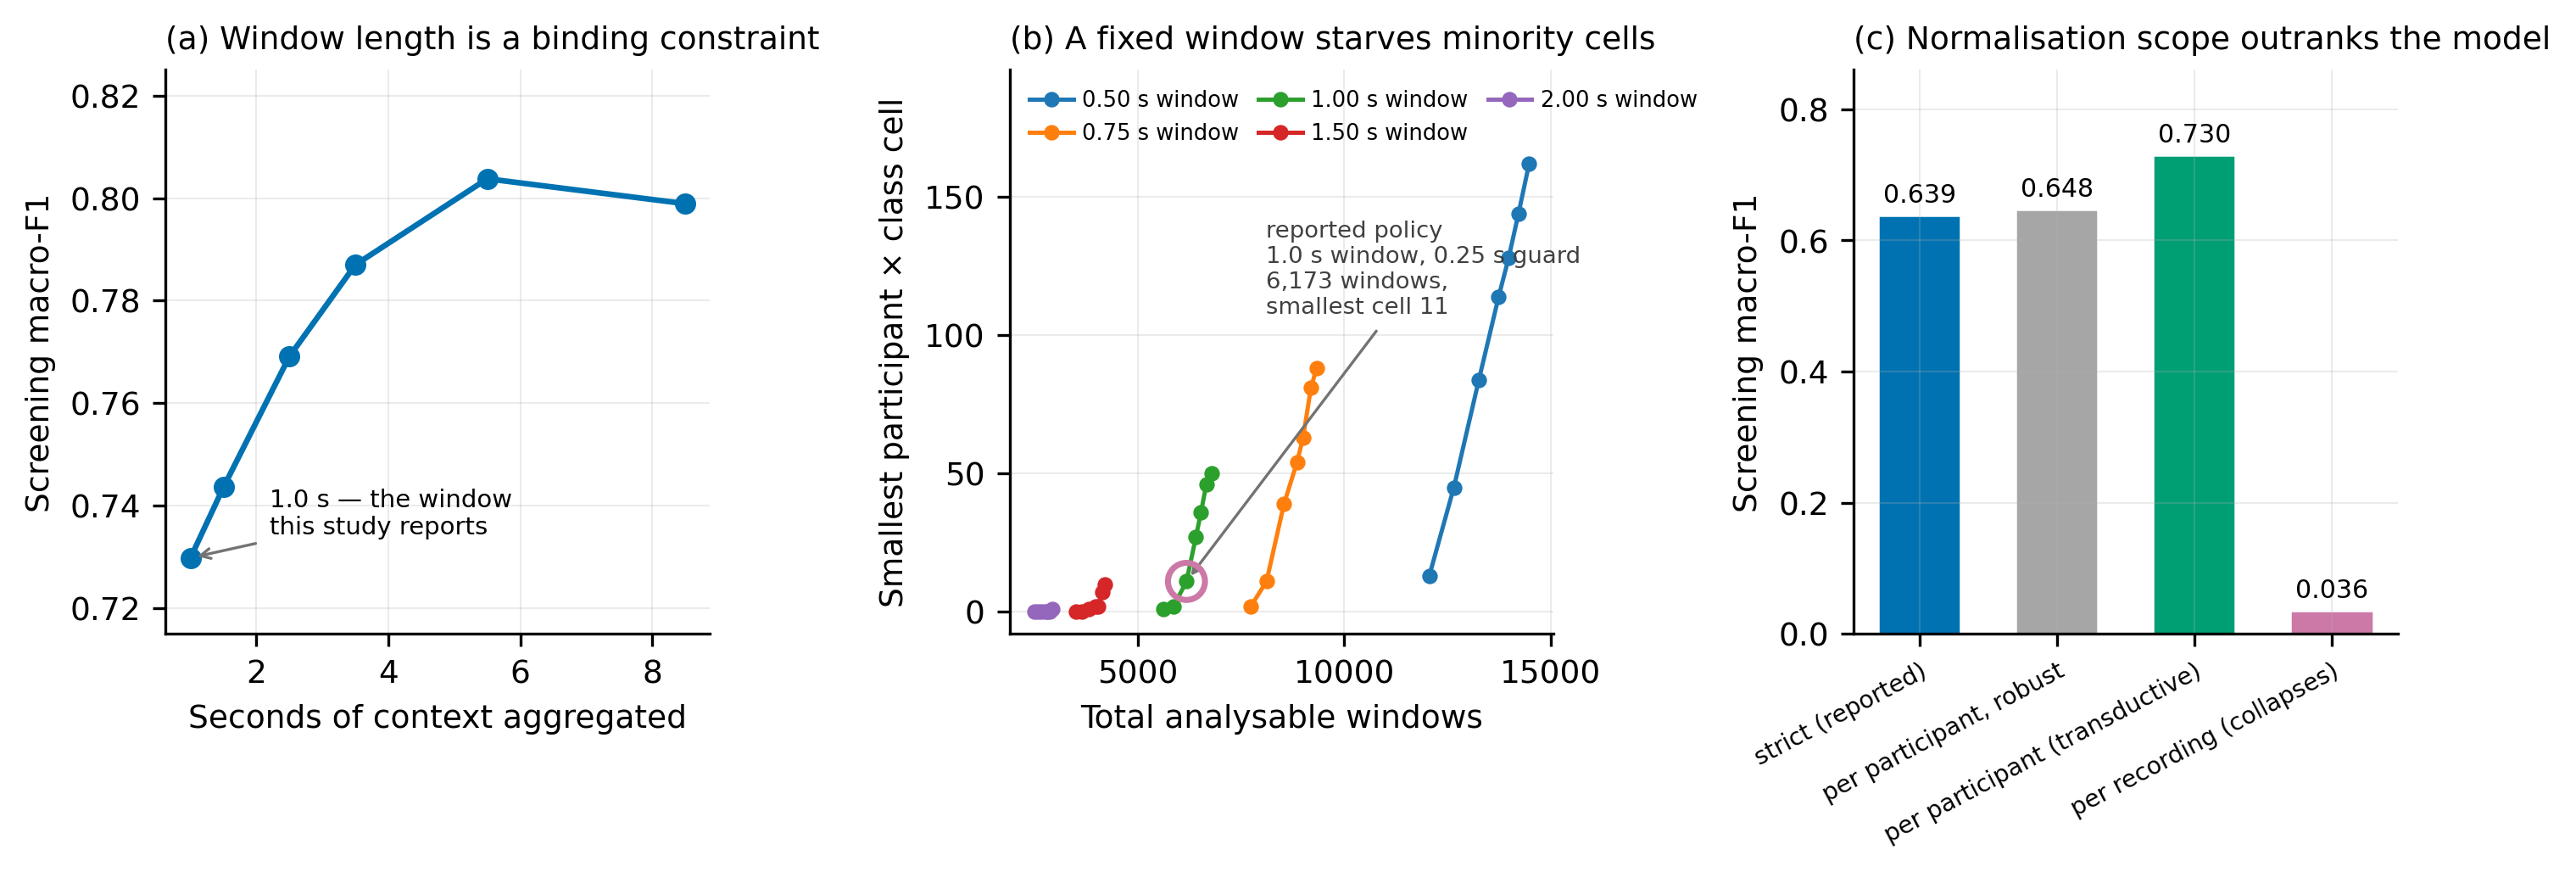
\includegraphics[width=0.88\linewidth]{Figures/v5/design_constraints.png}
  \caption{Three design constraints, all measured on identical windows and folds with the screening harness and the 28 EMG features. (a) Screening macro-F1 against seconds of temporal context aggregated within a recording; monotone across the range, so the 1.0-s window is a constraint rather than a tuned parameter. TRIAL-LEVEL: each recording holds one condition, so this is a labelled secondary analysis, not stream detection. (b) Every window/guard setting the audit swept: total analysable windows against the smallest participant $\times$ class cell, reported policy circled. The curves separate by window length because trigger granularity differed sharply between participants---67 runs of median 8.7~s for P1, 167 of 1.7~s for P2, 132 of 2.9~s for P3, 141 of 2.9~s for P4, 116 of 3.9~s for P5---so one rule emits very different counts from each. (c) Normalisation scope: the transductive per-participant scope is worth more than the architecture, and is used by no reported number.}
  \label{fig:design}
\end{figure*}

\subsection{Training behaviour and computational cost}
\label{sec:cost}

Because each fold's final model is refit for a fixed epoch budget chosen inside that fold, there is no early stopping and no validation set at refit time: the curves in Fig.~\ref{fig:loss_curves} are training-fit diagnostics and the held-out participant appears in none of them. Training loss had largely flattened by the end of each budget. The gap between final training-fit macro-F1 and the corresponding held-out macro-F1 averaged 0.144 and ranged from $-0.027$ to 0.291; per participant it was 0.276 for P1, 0.153 for P3, 0.129 for P4, 0.120 for P2 and 0.040 for P5. That ordering tracks the per-participant scores of Table~\ref{tab:persubject} almost exactly---the largest gap belongs to the participant whose windows are the most numerous and the least well ranked---the signature of between-participant variation rather than optimisation failure.

Three latencies must be kept separate. The \emph{input-context latency} is 1000~ms: the window length, and therefore the earliest point at which any decision can exist. The \emph{decision update interval} is 500~ms, the stride. The \emph{processing latency}---the forward pass for one pre-segmented window at batch size 1 on an Intel CPU---has a median of 1.02~ms and a 95th percentile of 1.06~ms, rising to 1.24~ms once amortised per-window preprocessing is included, which puts the earliest possible decision at about 1001~ms. The same bench measures the other three architectures of Table~\ref{tab:architectures} on the same four channels: 0.20~ms for the early-fusion CNN, 1.16~ms for the bidirectional LSTM, and 2.21~ms for the temporal CNN, whose modulation-spectrum head makes it the slowest of the four as well as the most accurate. Compute time alone is not detection latency, and none of these measurements supports a wearable or real-time claim: no streaming implementation exists, the production chain is zero-phase and therefore acausal, and the measurements were taken on laptop and desktop hardware. Power consumption, end-to-end latency, wireless synchronisation and wearable reliability remain unmeasured.

\begin{figure*}[t]
  \centering
  
\includegraphics[width=0.74\linewidth]{Figures/v5/training_curves_5class.png}
  \caption{Refit training loss (a) and training-fit macro-F1 (b) for all fifteen fold--seed combinations, coloured by held-out participant; line style encodes seed (solid 0, dashed 1, dotted 2). Each refit runs for the epoch budget chosen inside its own fold, so curves end at different epochs. The held-out participant contributes to no curve and is scored once, after training ends.}
  \label{fig:loss_curves}
\end{figure*}

\section{Discussion}

\subsection{The measurement finding}

On these recordings, whether the mains harmonics were removed determined more about what a classifier could learn than the architecture, the loss function, the feature set or the estimator. This is not merely a story about one bad filter. The defect was not a coding error, and no amount of testing would have caught it: the code implemented exactly the filter it was asked for, the filter was the one the literature recommends~\cite{chowdhury2013surface,raez2006techniques}, and its response plot is textbook-correct in isolation. What was missing was one comparison---the filter response drawn over the measured spectrum of the actual recordings---and one statistic, the share of in-band power sitting within a few hertz of each mains multiple. Both cost a single pass over the data, and neither appears in the studies this work is compared against, so a reader has no way to tell whether a published accuracy in this area describes physiology or interference.

How the defect presented deserves as much attention as its size. It did not look like a signal problem. It looked like between-participant heterogeneity---two of five held-out participants near chance, three in the normal range, a spread of 70 points of macro-F1---which is the most familiar failure mode in this literature and the one that motivates transfer learning, per-user calibration and larger cohorts. All three would have been reasonable responses, and none would have worked. A defect in a shared measurement chain expresses itself as apparent variation between the people measured through it, because interference amplitude varies with electrode impedance, cable routing and session rather than with physiology~\cite{deluca2010filtering,besomi2019consensus}, and LOSO then attributes that variation to the person held out. It presents, in other words, as precisely the input-distribution shift that the domain-generalisation literature sets out to absorb~\cite{wang2022generalizing,kouw2021review}---which is why the natural responses are the wrong ones here. The shift was a property of the instrument, not of the people, and no amount of adaptation to it would have recovered a signal the filter had already passed through untouched. This failure mode is adjacent to, but distinct from, the leakage and validation errors catalogued in clinical machine learning~\cite{saeb2017need,kapoor2023leakage,varoquaux2022machine}: nothing leaked and the protocol was correct; the input was not.

\subsection{The classification finding, and what bounds it}

On the corrected signal, four channels of surface EMG and 5,901 parameters separate five instructed experimental conditions under a protocol in which no held-out participant's windows touched normalisation, class weighting, augmentation or training. Quiet rest---the class added to test whether activity can be scored against a non-event condition rather than only against other activities---proved the most reliably recovered class of the five. The residual 7.7\% of rest windows assigned to clenching or grinding is the most decision-relevant number in the paper, because it is the closest available analogue of a false alarm.

The architectural claim is real but bounded, and its most interesting property is that it is contingent. The network beats the band energies it is built from on macro-F1 but not on AUC, where a linear model on those same features ranks held-out windows equally well: what it buys is better-placed decision boundaries, not better ordering. Through the defective chain even that comparison was a tie, for the reason given in Section~\ref{sec:rq3}. Architectural comparisons are therefore conditional on signal quality in a way that is rarely stated, and an architecture can be dismissed on the strength of a measurement defect.

The sweep against other learned architectures bounds the claim further, and in this paper's own direction. The reported network beats an early-fusion CNN on the raw signals and a bidirectional LSTM, both of them larger than it, so the wavelet decomposition does work that capacity alone does not replace. But a variant of the same front end that can represent burst--relaxation rhythm beats the reported network in turn---consistently across seeds, though on three of five participants and at three times the parameters. Both results point the same way: what separated these architectures was which information each could represent, not how many parameters it had, and the most valuable piece of information, rhythm over more than one second, is the one Section~\ref{sec:constraints} prices as a property of the recording design rather than of the model. The measurement finding reaches that conclusion by a different route.

The chewing class deserves the same double reading. It supplied most of the windows and achieved the highest F1 of any class, and excluding it lowered participant-level accuracy while raising macro-F1. The direction of those two changes is the point: a headline accuracy over this class distribution is carried substantially by the easiest and largest class, whereas macro-F1 rises once that class is removed because the remaining four are more evenly sized. Reporting both analyses, and macro-F1 alongside accuracy throughout, is what stops the largest class carrying the summary. The clenching--grinding split was retained for a related reason: clenching is static isometric loading and grinding is lateral excursion under load~\cite{lan2022comparative}, and a system meant to characterise tooth-contact activity should be tested on whether it resolves them rather than credited for collapsing them. It is also the hardest distinction in the problem, and a 1-second window from a grinding bout passing through a static phase may legitimately carry either label, so part of that confusion is label ambiguity rather than model error.

Comparison with the greater-than-90\% accuracy reported by Sonmezocak and Kurt using EMG alone~\cite{sonmezocak2021detection} is not like-for-like: their classes were jaw opening, clenching, rhythmic grinding and fatigue/pain against our five, and dataset composition, preprocessing, sample size and validation design all differ. Every number here is measured on a participant the model has never seen; a within-participant or window-shuffled split of the same data would score considerably higher without measuring anything about a new user~\cite{saeb2017need,little2017using}. The two studies answer different questions.

\subsection{What a next study should do}

Section~\ref{sec:constraints} priced three choices this design fixed early, and two proved worth more than the architecture---the practical message for anyone planning a follow-on collection. Temporal context is the clearest: performance rises monotonically from 1.0 to 5.5~s, so the 1-second window is a limitation of this analysis rather than an optimum it found. A next-stage design should classify variable-length segments directly or aggregate over a declared context, and must then evaluate on continuously varying activity rather than single-condition trials, because the aggregation measured here is a majority vote over a homogeneous trial and cannot be presented as event detection. Trigger granularity is the least obvious constraint and the easiest to fix: because participants marked bouts as they saw fit, one produced seven times as many clenching windows as another from the same instructed task, and the smallest participant $\times$ class cell holds 11 windows. That is an instruction problem, not a modelling one, removable at source by standardising trigger use, by recording continuous condition intervals rather than participant-marked bouts, or both.

Normalisation scope, finally, is a product decision disguised as a preprocessing one: standardising by the held-out participant's own unlabelled distribution uses no labels and is entirely legitimate, but it presumes a per-user fitting session and therefore describes a device the user calibrates rather than one that works immediately. We report the strict scope throughout because it supports the weaker and more defensible claim, and report the gap so that a future design can decide deliberately rather than by default~\cite{besomi2020consensus}.

Setting is the remaining gap. Laboratory repetitions do not capture the frequency, duration or day-to-day variability of behaviour outside the laboratory, and awake bruxism is currently characterised mainly by ecological momentary assessment rather than by any instrument~\cite{bracci2018frequency}, while multi-day, 24-hour home EMG recording has been shown to be feasible and illustrates its own difficulties~\cite{colonna2023electromyographic,lobbezoo2020consensus}. A next-stage awake study should therefore combine multi-day EMG with a clearly defined background class and blinded annotation of candidate episodes, and should report day-level and participant-level performance including false positives per hour. No conclusion about sleep follows from these awake laboratory tasks: a sleep study would require overnight data, appropriate sleep staging and event criteria, comparison with a suitable reference such as polysomnography or validated portable assessment, and repeated nights to evaluate night-to-night variability~\cite{lavigne1996sleep,casett2017validity,cidverdejo2024instrumental}. Separate models may be required for awake and sleep contexts.

\subsection{Why the microphone was excluded, and what would make it answerable}
\label{sec:mic_discussion}

Two points about the exclusion deserve emphasis. First, the defect is invisible from any single recording: every affected file is individually well-formed, correctly sized and carries plausible values, and the duplication appears only when two files are compared. An audit that examines recordings one at a time therefore cannot detect it, which is precisely why our own first audit---thorough, reproducible and pointed at the electromyogram---did not reach it. The check that does is cheap and modality-agnostic: a rotation-invariant fingerprint of every channel of every recording, grouped, with a refusal if any held-out participant's signal appears in its own training set.

Second, this determines what may be said next. An underpowered result and an invalid input are different problems with different remedies: more participants would address the first, only a new acquisition the second. We therefore report neither a weak fusion benefit nor a finding that a microphone does not help; the honest position is that the question is untested. Answering it would require a documented transducer with a stated frequency response and output type, a sampling rate matched to the band in which tooth contact actually radiates~\cite{romano2024wearable}, verified time alignment against the electromyogram, and a per-recording channel-integrity check run before any model is fitted. Figure~\ref{fig:signal_comparison} shows what the electromyogram alone contains for the three conditions in question.

\begin{figure*}[t]
  \centering
  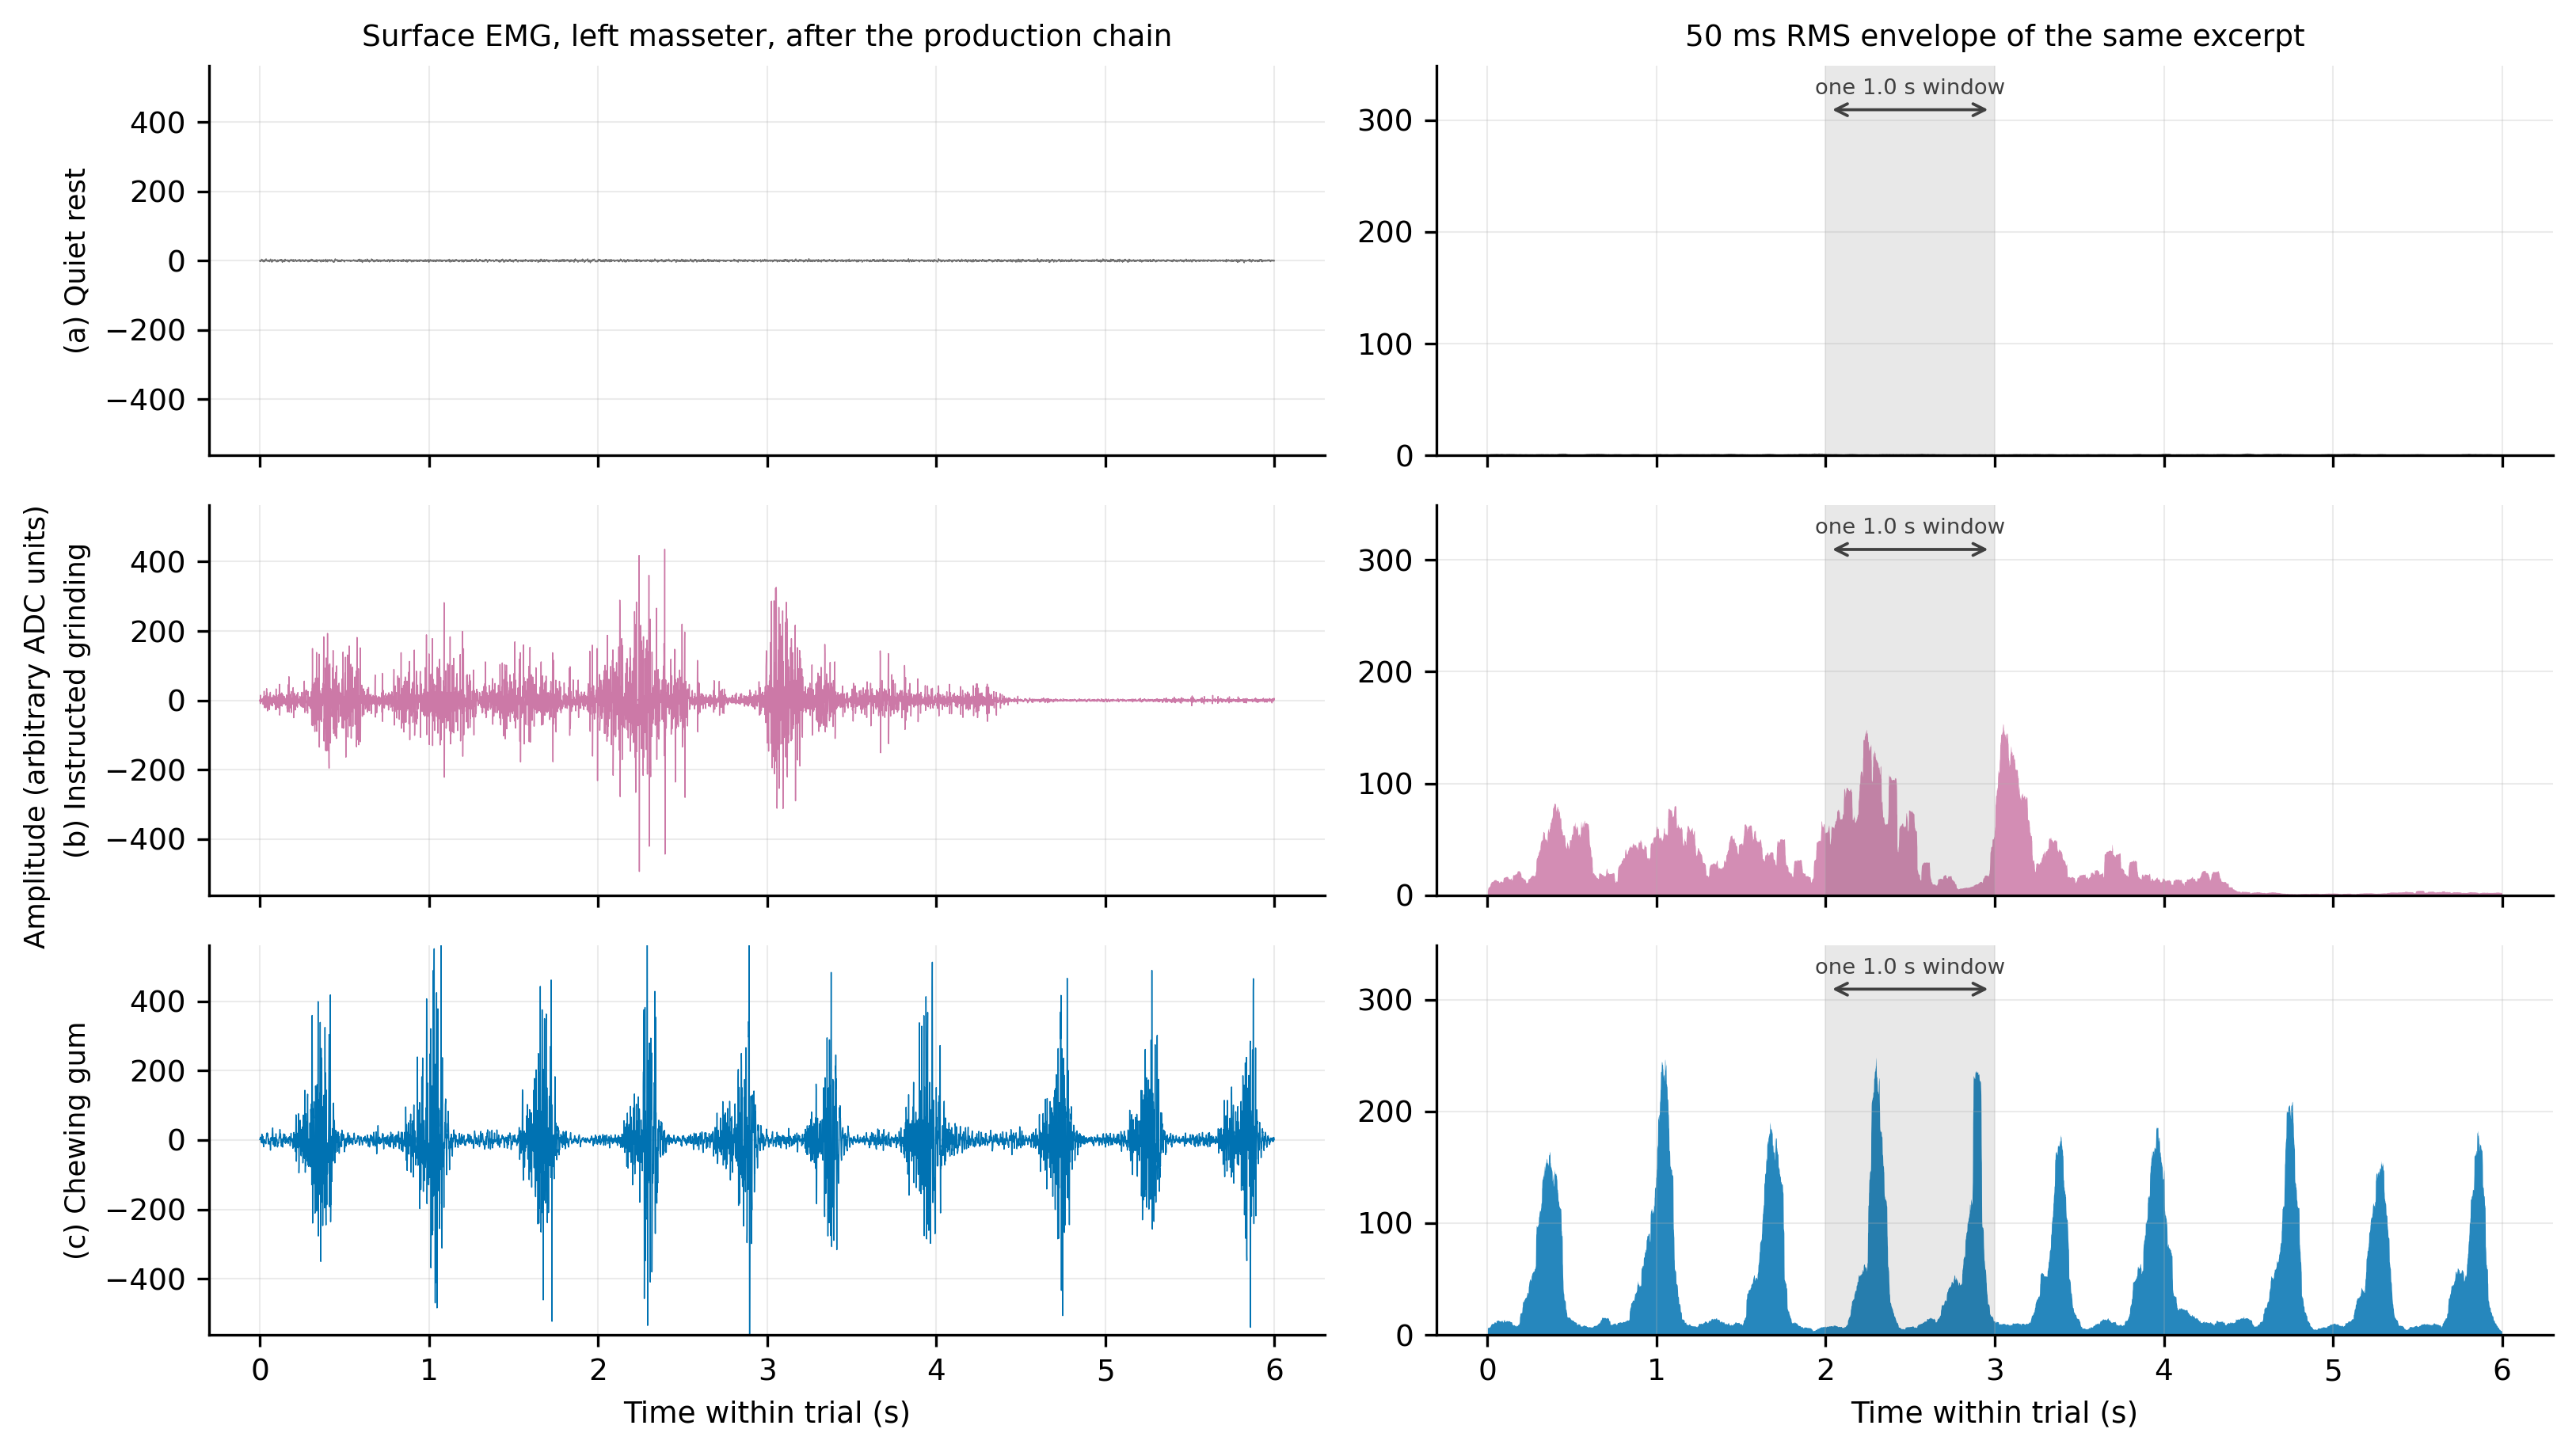
\includegraphics[width=0.78\linewidth]{Figures/v5/signal_comparison_emg.png}
  \caption{Six-second excerpts of one participant's quiet rest, instructed grinding and gum chewing after the corrected chain, on a common scale, with the 50~ms RMS envelope beside each. (a) Rest is quiet. (b) Grinding produces sustained activation without a clear burst--relaxation rhythm. (c) Chewing produces rhythmic bursts separated by relaxation intervals at roughly 1.4~Hz. The shaded interval is one 1.0-second analysis window to scale: it holds barely one chewing cycle, the constraint quantified in Fig.~\ref{fig:design}a.}
  \label{fig:signal_comparison}
\end{figure*}

\subsection{Validity and limitations}

The principal limitation is the cohort size ($N=5$). The 6,173 overlapping windows supply many optimisation examples but do not replace independent participants: adjacent windows share half their samples and one participant contributed 27\% of them. Window-level confidence intervals or tests would overstate precision and are deliberately not reported, and LOSO does not establish external generalisation from five people~\cite{varoquaux2018cross}. The between-participant spread is itself the clearest evidence that a five-person mean is not a population estimate, and age, facial anatomy, subcutaneous tissue, dentition, electrode placement, skin impedance, behaviour intensity and prior diagnosis may all affect the signal~\cite{besomi2019consensus,hermens2000development}.

The RQ1 contrast likewise comes from one cohort in one laboratory, and its magnitude is not a general effect size for mains correction: what generalises is the mechanism and the check, not the 29.3 points. Two features bound it in opposite directions. Both arms are the fused condition, so the superseded arm carried an extra input channel and additionally searched its loss and learning rate, making the gap conservative; but the two runs differ in codebase version, and although the window set, fold assignment and labels are byte-identical and were verified as such, we cannot exclude an unrecorded contributing difference. The screening arms, which share one code path across both chains, move by a similar amount and are the cleaner evidence there. Some declared options were also left unexercised: temperature scaling is implemented but unapplied, so held-out scores must not be read as probabilities~\cite{guo2017calibration} though every AUC is unaffected, and the per-participant normalisation scope and temporal aggregation of Section~\ref{sec:constraints} are excluded from every reported result for the reasons given there.

Task coverage and label precision bound what the classes mean. The tasks cover tooth-contact clenching and grinding but not bracing or thrusting without tooth contact~\cite{verhoeff2025definitions}, and the prior diagnoses were not phenotyped for this study~\cite{manfredini2024standardised}. Class membership rests on a button press confirmed by the experimenter: muscle activity preceded the marker at four of every five onsets, and while the 0.25-s guard exceeds the median error in the harmful direction and covers the 95th percentile, 7\% of trial-leading windows may still carry a partially mislabelled edge. The grinding condition's acquisition token was a filename label chosen at recording time, so that class is reported throughout as instructed grinding. Because every activity was performed on instruction, it may be more regular, longer or more forceful than spontaneous activity---a bias in the optimistic direction~\cite{farella2008masticatory}---and no spontaneous episode was verified against a reference standard.

Including quiet rest removes one limitation of an activity-only design, but the background data remain incomplete. Rest was recorded in a controlled laboratory and did not systematically sample speaking, swallowing, facial expression, head movement, coughing, eating outside the scripted task, environmental noise or other free-living behaviour. The five-class analysis can therefore estimate confusion against quiet rest but not false alarms per hour during unrestricted use, because the denominator that matters there is unrestricted behaviour and this design contains none. Finally, the computational measurements were taken on laptop and desktop hardware rather than a wearable prototype, and the acausal filter chain means they do not describe a streaming system.

\section{Conclusion}

This five-participant proof-of-concept study asked what a compact wavelet convolutional network can do with four channels of surface EMG, and found first that the answer depends more on the measurement chain than on the network. Because the acquisition hardware had already removed the 60-Hz fundamental and the surviving interference was harmonic, the conventional chain was indistinguishable in effect from applying no mains filter at all; replacing it with a constant-width harmonic notch bank moved the matched nested-LOSO network by 29.3 points of participant-level macro-F1 on byte-identical windows, folds and labels, and two much simpler classifiers by 22 to 27. On the corrected signal the model reached 81.7\% accuracy and 72.0\% macro-F1 in 5,901 parameters, with quiet rest the best-recalled class, and beat hand-engineered band energies from the same bands by a margin that did not exist before the correction---and is therefore a property of the corrected signal as much as of the architecture.

The transferable recommendation is procedural and costs one pass over the data. Report a measured interference statistic beside every accuracy, and draw filter responses over the measured spectrum of the recordings rather than alone. Fingerprint every channel of every recording---a hash of its sorted samples suffices, and is invariant to the circular rotation that hid the second defect here---then group the fingerprints and confirm that no held-out participant's signal appears in its own training set. Defects of both kinds are invisible in any single file and in any amount of unit testing: the code is correct, the pipeline reproducible and the figures right, because nothing in the figure set compares the analysis to the data it was applied to.

This study does not validate a bruxism detection device. Quiet-rest windows are included, but there is no bracing or thrusting, no unrestricted background behaviour, no spontaneous awake episode, no sleep recording and no independent reference standard. The defensible conclusion is technical: surface EMG with modality-specific wavelet decomposition merits further evaluation for distinguishing instructed jaw activities from quiet rest, in a larger, phenotyped, multi-day continuous-recording study---and any such study should publish the measured properties of its signals alongside the accuracy it obtained from them.

\backmatter

\section*{Data availability}
The datasets generated and/or analysed during the current study are not publicly available because of participant-privacy restrictions but are available from the corresponding author on reasonable request, subject to institutional and ethical requirements.

\section*{Code availability}
The custom code used for signal preprocessing, wavelet decomposition, model training and evaluation is available from the corresponding author on reasonable request. Every number and figure in this manuscript was regenerated from a saved artifact rather than transcribed. The confirmatory five-class results come from the EMG conditions of run \texttt{modality\_and\_no\_chewing\_}\allowbreak\texttt{20260810T020642\_cead62e4}, configuration hash \texttt{cead62e4}, manifest hash \texttt{7ebbcc8d}, window-index hash \texttt{b2cf690c}. The architecture sweep of Section~\ref{sec:deep_baselines} comes from run \texttt{baselines\_emg\_only\_20260816}, which carries a different manifest hash (\texttt{9d93667b}) and window-index hash (\texttt{9941fe48}) because the manifest schema was extended, after the microphone audit, with the channel-integrity columns and the cross-recording fingerprint pass described in Section~\ref{sec:mic}. The window set is nevertheless the same one: comparing the two prediction ledgers window by window returns the identical 6,173 windows, the identical class labels and the identical held-out-participant assignment, with no window present in one and absent from the other. Each prediction ledger records every held-out window exactly once per task, modality and seed, together with its full probability vector, the source commit, and hashes of the resolved configuration, the data manifest, the window index and the model checkpoint. The screening measurements for RQ1, RQ3 and Section~\ref{sec:constraints} come from the same window index, so every comparison in this paper was evaluated on the identical set of windows. Run bundles retain the hashes they were produced under and still reproduce. The participant-level values in Table~\ref{tab:architectures} were recomputed from that run's saved prediction ledgers into \texttt{outputs/}\allowbreak\texttt{summaries/}\allowbreak\texttt{baselines\_emg\_only\_}\allowbreak\texttt{20260816}, and the parameter counts and latencies in Table~\ref{tab:architectures} and Section~\ref{sec:cost} from \texttt{outputs/benchmarks/}\allowbreak\texttt{benchmark\_emg\_only.json}, measured on the four EMG channels through the corrected filter chain on an otherwise idle machine. An earlier benchmark of the fusion variants, taken before the filter correction, is retained but is not the source of any number reported here.

\section*{Funding declaration}
Research reported in this publication was supported by an award from the Rhode Island Life Science Hub Small Grant Program (Principal Investigator T. A. Walls; Co-Investigators R. Abiri and M. Furmanek). The project was also partially supported by National Science Foundation grant 2245558 (Principal Investigator R. Abiri).

\section*{Acknowledgements}
We thank University of Rhode Island undergraduate and graduate students Anjolaoluwa Akingbile, Jessica Constantine and Nathan DeSalvo, who located and summarised the functions of bruxism devices before this project.

\section*{Author contributions}
M.H.F.: methodology, software, analysis, writing---original draft, and writing---review and editing. A.R.: protocol development, software, data curation, data collection, formal analysis, and review and editing. R.S.: methodology, validation, and writing---review and editing. M.P.F.: conceptualization and study design, research-grant development, protocol development, and manuscript revision. R.A.: conceptualization, project administration, resources, supervision, and writing---review and editing. T.A.W.: conceptualization, research-grant authorship, protocol development, project oversight, and manuscript revision. All authors reviewed and approved the final manuscript.

\section*{Competing interests}
The authors declare no competing interests.

\bibliography{refs}

\end{document}
